\documentclass[a4paper,11pt,italian]{article}
\usepackage[T1]{fontenc}
\usepackage[utf8]{inputenc}
\usepackage[italian]{babel}
\usepackage{amsmath}
\usepackage{mathrsfs}
\usepackage{hyperref}

%%%--- impostazioni font
\usepackage{sansmathfonts}
\usepackage[scaled=0.85]{helvet}
\renewcommand{\rmdefault}{\sfdefault}
\usepackage[font=footnotesize,width=.75\textwidth]{caption}

%%%--- frazioni carine \sfrac{}{}
\usepackage{xfrac}

%%%--- interlinea
\usepackage{setspace}
\setstretch{1.3}

%%%--- multicolonna
\usepackage{multicol}

%%%--- figure in orizzontale
\usepackage{rotating}

%%%--- margini e bordo
\usepackage[margin=2.7cm]{geometry}
% \usepackage{showframe}

%%%--- impostazioni tikz e grafici
\usepackage{pgf,tikz,pgfplots,bm,pgf-spectra,graphicx,timelines}
\usepackage{circuitikz}
\usetikzlibrary{angles,quotes,arrows,shapes,decorations.markings}
\tikzset{fleche/.style args={#1:#2}{postaction=decorate,decoration={name=markings,mark=at position #1 with {\arrow[#2,scale=1.5]{latex}}},},}
\pgfplotsset{compat=1.15}
\usepgfplotslibrary{units,fillbetween}

%%%--- info documento
\title{\textbf{\Huge \color{colorSitoScuro}Formulario di Fisica}}
\author{\LARGE \color{colorSitoScuro}Mattia Cozzi}
\date{}

%%%--- riferimenti intelligenti
\usepackage[noabbrev]{cleveref} %opzione capitalize per tutto maiuscolo

%%%---righelli migliori per tabelle
\usepackage{booktabs}

%%%--- impostazioni dei colori
\usepackage{xcolor}
\usepackage{sectsty}
\usepackage{enumitem}
%%%--- TEAL
% \definecolor{colorSito}{rgb}{.04,.212,.22}
% \definecolor{colorSitoChiaro}{rgb}{.20,.408,.416}
% \definecolor{colorSitoScuro}{rgb}{.0,.133,.141}
%%%--- BORDEAUX
\definecolor{colorSito}{rgb}{.612,.067,.192}
\definecolor{colorSitoChiaro}{rgb}{.69,.145,.271}
\definecolor{colorSitoScuro}{rgb}{.22,.0,.0}

\sectionfont{\color{colorSito}}  %imposta il colore delle sezioni
\subsectionfont{\color{colorSitoChiaro}}  %imposta il colore delle sottosezioni
\subsubsectionfont{\color{colorSitoChiaro}}  %imposta il colore delle sottosottosezioni
\setlist[description]{format=\textcolor{colorSitoScuro}} %imposta il colore degli elementi di una lista di definizione

%%%--- nuovi comandi


%%%---cerca NON NECESSARIO per trovare le formule commentate
\begin{document}

%%%---indice
\maketitle
\vspace{8em}
\tableofcontents

\newpage
\section{Vettori}

\begin{description}
  \item[Scalari e vettori] 
  Una grandezza può:
\begin{itemize}
  \item essere espressa completamente tramite un valore numerico, come la massa: è uno \emph{scalare};
  \item richiedere l'esplicitazione anche di una direzione e di un verso, come la velocità o la forza: è un \emph{vettore}.
\end{itemize}
  Gli scalari sono indicati con lettere, i vettori con lettere sormontate da una freccia, come $ \vec{a} $.
  
  Il modulo del vettore $ \vec{a} $ viene indicato con $ |a| $ o più semplicemente con $ a $.
  
  \item[Versore]
  Un versore è un vettore di modulo $ 1 $. Vengono indicati con i simboli $ \hat{i}  $, $ \hat{j} $, $ \hat{k} $, $ \hat{n} $, ecc.
  
  I versori possono essere usati per rappresentare la direzione e il verso di un vettore, indicando poi con uno scalare il modulo.
  
  Ad esempio, $ \vec{a} = 5\hat{i}  $ indica un vettore $ \vec{a} $ con la stessa direzione e verso del versore $ \hat{i} $ e di modulo $ 5 $.
  
  Solitamente i versori $ \hat{i}  $, $ \hat{j} $ e $ \hat{k} $ sono usati per indicare gli assi cartesiani, 
  mentre con $ \hat{n} $ si indica un versore normale (perpendicolare) ad un piano.
  
  \item[Funzioni goniometriche (seno, coseno, tangente)]
  In un triangolo rettangolo, possiamo distinguere i due cateti in \emph{cateto opposto all'angolo $ \theta $} 
  e \emph{cateto adiacente a $ \theta $}, in base alla posizione che occupano rispetto all'angolo $ \theta $.
  
  Definiamo le seguenti funzioni goniometriche:
\begin{multicols}{3}
  \begin{center}
  $ \cos\theta = \dfrac{c_{adj}}{i} $
  
  $ \sin\theta = \dfrac{c_{opp}}{i} $
  
  $ \tan\theta = \dfrac{c_{opp}}{c_{adj}} $
  \end{center}
\end{multicols}
  \begin{figure}[htb]\centering
  \begin{tikzpicture}
  \draw (0,0) -- (4,0);
  \node [below] at (2,0) {$ c_{adj} $};
  \draw (4,0) --(4,3);
  \node [right] at (4,1.5) {$ c_{opp} $};
  \draw (4,3) -- (0,0);
  \node [above left] at (2,1.5) {$ i $};
  \draw (0.4,0) arc [start angle=0,end angle=37,radius=0.4] node[pos=0.8,right]{$\theta$};
  \end{tikzpicture}\caption{Notiamo che, essendo l'ipotenusa sempre maggiore di ognuno dei due cateti, seno e coseno di un angolo sono valori con modulo minore di 1.}
  \end{figure}
  
  Quando si eseguono calcoli con le funzioni goniometriche, assicurarsi che gli angoli siano espressi con l'unità di misura desiderata. 
  La calcolatrice dovrà riportare esplicitamente \colorbox{black}{\textcolor{white}{D}} per i gradi (\emph{degrees}) o \colorbox{black}{\textcolor{white}{R}} per i radianti (possiamo ignorare la dicitura \colorbox{black}{\textcolor{white}{G}}).
  
  \item[Scomposizione di un vettore]
  Una volta stabilito un sistema di riferimento, possiamo determinare l'angolo che un vettore $ \vec{a} $ forma con l'asse $ x $ (la cui direzione è data dal versore $ \hat{i} $).
  
  Chiamiamo tale angolo $ \theta $ e calcoliamo le componenti cartesiane del vettore (ovvero le sue proiezioni sugli assi cartesiani) utilizzando le formule precedenti:
  \[ a_x = a  \cos\theta \quad\quad\quad\quad a_y = a  \sin\theta \]
  
    \begin{figure}[htb]\centering
    \begin{tikzpicture}[>=latex]
    \draw [dashed] (4,0) --(4,3);
    \draw [dashed] (0,3) -- (4,3);
    \draw [->](-.5,0) -- (5,0);
    \draw [->](0,-.5) -- (0,4);
    \draw [colorSitoChiaro!50,thick](.7,0) arc [start angle=0,end angle=37,radius=.7,thick] node[pos=0.8,right]{$\theta$};
    \node [below] at (5,0) {{\small $ x $}};
    \node [left] at (0,4) {{\small $ y $}};
    \node [below] at (4,0) {{\small $ a_x $}};
    \node [left] at (0,3) {{\small $ a_y $}};
    \draw [->,ultra thick,colorSito!80](0,0) -- (4,0);
    \draw [->,ultra thick,colorSito](0,0) -- (4,3);
    \node [left,colorSito] at (0,1.5) {$ \vec{a}_y $};
    \node [below,colorSito!80] at (2,0) {$ \vec{a}_x $};
    \draw [->,ultra thick,colorSito!80] (0,0) -- (0,3);
    \node [above left,colorSito] at (2,1.5) {$ \vec{a} $};
    \node [left,colorSitoScuro] at (-.07,.8) {$ \hat{j} $};
    \node [below,colorSitoScuro] at (.8,-.07) {$ \hat{i} $};
    \draw [line cap=round,->,ultra thick,colorSitoScuro] (0,0) -- (1,0);
    \draw [line cap=round,->,ultra thick,colorSitoScuro] (0,0) -- (0,1);
    \end{tikzpicture}
    \caption{La scomposizione di un vettore nelle sue componenti lungo gli assi cartesiani (determinati dai versori $ \hat{i} $ e $ \hat{j} $).}
    \end{figure}
  
  
  Possiamo ora esprimere il vettore $ \vec{a} $ mediante le sue componenti sugli assi.
  \[ \vec{a} = a_x \hat{i} + a_y \hat{j} \]
  
  \item[Modulo e direzione di un vettore, note le componenti]
  Dato un vettore $ \vec{a} = a_x \hat{i} + a_y \hat{j}  $ possiamo risalire al suo modulo con il teorema di Pitagora:
  \[ a = \sqrt{(a_x)^2 + (a_y)^2} \]
%   Per ottenere l'angolo  formato con l'asse $ x $ possiamo usare una tra le seguenti formule (che utilizzano le funzioni inverse delle funzioni goniometriche):
%   \[ \theta  = \arccos\left( \frac{a_x}{a} \right) = \arcsin\left( \frac{a_y}{a} \right) = \arctan\left( \frac{a_y}{a_x} \right) \]
%   Sulle calcolatrici scientifiche, le funzioni inverse delle funzioni goniometriche sono solitamente indicate come $ \cos^{-1} $, $ \sin^{-1} $ e $ \tan^{-1} $.
\end{description}

\subsection{Operazioni coi vettori}

\begin{description}
  \item[Somma tra vettori, metodo grafico]
  Regola del parallelogramma, mostrata in \Cref{img:parallelogramma}.

\begin{figure}[htb]\centering
\begin{tikzpicture}[>=latex]
\draw [dashed] (0,0) -- (2,3);
\draw [dashed] (2,3) -- (6,3);
\draw [line cap=round,->,colorSito!70,ultra thick] (0,0) -- (4,0);
\node [below,colorSito!70] at (2,0) {$ \vec{a} $};
\draw [line cap=round,->,colorSito!70,ultra thick] (4,0) -- (6,3);
\node [below right,colorSito!70] at (5,1.5) {$ \vec{b} $};
\draw [line cap=round,->,colorSito,ultra thick] (0,0) -- (6,3);
\node [below right,colorSito] at (3,1.5) {$ \vec{c} $};
\end{tikzpicture}\caption{Regola del parallelogramma: $ \vec{a} + \vec{b} = \vec{c} $.}
\label{img:parallelogramma}
\end{figure}

  \item[Somma tra vettori, metodo algebrico]
  Dati due vettori $ \vec{a} = a_x \hat{i} + a_y \hat{j} $ e  $ \vec{b} = b_x \hat{i} + b_y \hat{j} $ il vettore somma sarà: 
  \[ \vec{a} + \vec{b} =  (a_x + b_x) \hat{i} + (a_y + b_y) \hat{j}  \]
  È sufficiente sommare le componenti sui rispettivi assi.
  
  \item[Differenza tra vettori]
  Graficamente, basta invertire il verso del vettore da sottrarre e procedere come per la somma. Il metodo del parallelogramma viene applicato come in \Cref{img:parallelogramma2}.

\begin{figure}[htb]\centering
\begin{tikzpicture}[>=latex]
\draw [dashed] (4,0) -- (2,-3);
\draw [dashed] (-2,-3) -- (2,-3);
\draw [line cap=round,->,colorSito!70,ultra thick] (0,0) -- (4,0);
\node [below,colorSito!70] at (2,0) {$ \vec{a} $};
\draw [line cap=round,->,colorSito!70,ultra thick] (4,0) -- (-2,-3);
\node [below right,colorSito!70] at (1,-1.5) {$ -\vec{b} $};
\draw [line cap=round,->,colorSito,ultra thick] (0,0) -- (-2,-3);
\node [above left,colorSito] at (-1,-1.5) {$ \vec{c} $};
\end{tikzpicture}\caption{Regola del parallelogramma applicata alla sottrazione: $ \vec{a} + (-\vec{b}) = \vec{c} $.}
\label{img:parallelogramma2}
\end{figure}
  Algebricamente:
  \[ \vec{a} - \vec{b} =  (a_x - b_x) \hat{i} + (a_y - b_y) \hat{j} \]

  \item[Attenzione!]
  La moltiplicazione è un'operazione che ha senso solo su numeri (scalari). Quando abbiamo a che fare con dei vettori, parliamo di ``prodotto tra vettori''. 
  
  Esistono tre tipi di prodotto che utilizzano i vettori. In nessun caso dobbiamo leggere i simboli $ \cdot $ e $ \times $ come dei ``per''.
  
  \item[Prodotto di uno scalare per un vettore]
  Il prodotto di uno scalare per un vettore è un vettore che ha:
  \begin{itemize}
    \item la stessa direzione del vettore;
    \item stesso verso del vettore se lo scalare è positivo, verso opposto se lo scalare è negativo;
    \item modulo uguale al prodotto dello scalare per il modulo del vettore.
  \end{itemize}
  Intuitivamente, se eseguo il prodotto tra lo scalare $ 3 $ e il vettore $ \vec{a} $, otterrò un vettore orientato come $ \vec{a} $ ma tre volte più lungo.

\begin{figure}[htb]\centering
\begin{tikzpicture}[>=latex]
\draw [line cap=round,->,colorSitoChiaro,ultra thick] (0,0) -- (2,0);
\node [above,colorSitoChiaro] at (1,0) {$ \vec{a} $};
\draw [line cap=round,->,colorSitoScuro,ultra thick] (0,-.66) -- (6,-.66);
\node [above,colorSitoScuro] at (3,-.66) {$ 3\vec{a} $};
\end{tikzpicture}\caption{Prodotto del vettore $ \vec{a} $ per lo scalare $ 3 $.}
\label{img:prodottoscalarevettore}
\end{figure}

  Algebricamente: 
  \[ k \vec{a} = (k a_x)\hat{i} + (k a_y)\hat{j} \]
  Solitamente il prodotto di uno scalare per un vettore non viene indicato con alcun simbolo.
  
  \item[Prodotto scalare]
  Il prodotto scalare (simbolo $ \cdot $) si esegue tra due vettori e dà come risultato uno scalare.
  
  Si moltiplica il modulo del primo vettore per la componente del secondo lungo il primo (o viceversa: il prodotto scalare è commutativo), come mostrato in \Cref{img:scalare}.

\begin{figure}[htb]\centering
\begin{tikzpicture}[>=latex]
\draw [colorSitoChiaro!50,thick] (0.4,0) arc [start angle=0,end angle=57,radius=0.4] node[pos=0.2,above right,colorSitoChiaro!50]{$\theta$};
\draw [dashed,thick] (2,0) -- (2,3);
\node [below,colorSito] at (1,0) {$ b \cos \theta $};
\draw [line cap=round,->,colorSitoScuro,ultra thick] (0,0) -- (4,0);
\node [below,colorSitoScuro] at (2.5,0) {$ \vec{a} $};
\draw [line cap=round,colorSito,ultra thick] (-.05,-.05) -- (2,-.05);
\draw [line cap=round,->,colorSito,ultra thick] (-.05,-.05) -- (2,3);
\node [above left,colorSito] at (1,1.5) {$ \vec{b} $};
\end{tikzpicture}\caption{Rappresentazione della componente di $ \vec{b} $ su $ \vec{a} $.}
\label{img:scalare}
\end{figure}
  
  Se indichiamo con $ \theta $ l'angolo tra i due vettori $ \vec{a} $ e $ \vec{b} $, allora: 
  \[ \vec{a} \cdot \vec{b} = ab\cos\theta \]

%%%---NON NECESSARIO
%   Aggiungiamo che, conoscendo le componenti del vettore, è possibile dimostrare che vale: 
%   \[ \vec{a} \cdot \vec{b} = a_x b_x + a_y b_y \]
  
  \item[Prodotto vettoriale]
  Il prodotto vettoriale (simbolo $ \times  $) si esegue tra due vettori e dà come risultato un vettore.
  
  Il modulo del vettore $ \vec{a} \times \vec{b} $ è dato dall'area del parallelogramma costruito coi vettori $ \vec{a} $ e $ \vec{b} $.

\begin{figure}[htb]\centering
\begin{tikzpicture}[>=latex]
\fill[fill=colorSitoChiaro!10] (0,0) -- (4,0) -- (6,3) -- (2,3) -- cycle;
\draw [thick,colorSitoChiaro] (0.7,0) arc [start angle=0,end angle=57,radius=0.7] node[pos=0.2,above right]{$\theta$};
\draw [dashed,thick] (2,0) -- (2,3);
\node [right] at (2.05,1) {$ b \sin \theta $};
\draw [line cap=round,->,colorSitoScuro,ultra thick] (0,0) -- (4,0);
\node [below,colorSitoScuro,thick] at (2,0) {$ \vec{a} $};
\draw [dashed] (4,0) -- (6,3);
\draw [line cap=round,->,colorSitoScuro,ultra thick] (0,0) -- (2,3);
\node [above left,colorSitoScuro] at (1,1.5) {$ \vec{b} $};
\node [above left,colorSito] at (4,1.5) {$ |\vec{a}\times\vec{b}| $};
\draw [dashed] (2,3) -- (6,3);
\end{tikzpicture}\caption{Il modulo del prodotto vettoriale come area del parallelogramma.}
\label{img:vettoriale1}
\end{figure}
  
  Se indichiamo con $ \theta $ l'angolo tra i due vettori $ \vec{a} $ e $ \vec{b} $, allora: 
  \[ | \vec{a} \times \vec{b} | = ab\sin\theta \]

  Poiché il risultato dell'operazione è un vettore, dobbiamo ancora indicarne direzione e verso:
  \begin{itemize}
    \item la direzione del prodotto vettoriale di $ \vec{a} $ e $ \vec{b} $ è perpendicolare al piano da essi formato;
    \item il verso è dato dalla \emph{regola della mano destra}, ovvero ponendo il pollice della mano destra nel verso del vettore $ \vec{a} $ e le altre dita nel verso di $ \vec{b} $, il vettore $ \vec{a} \times \vec{b} $ sarà uscente dal palmo della mano, come indicato dalla \Cref{img:vettoriale2}.
  \end{itemize}
  
\begin{figure}[htb]\centering
\begin{tikzpicture}[>=latex]
\fill[fill=colorSitoChiaro!10] (0,0) -- (4,0) -- (3,-1) -- (-1,-1) -- cycle;
\draw (.3,0) -- (.3,.3);
\draw (.3,.3) -- (0,.3);
\draw (0,.3) -- (-.2,.1);
\draw (-.2,.1) -- (-.2,-.2);
\draw [colorSitoChiaro,thick](0.4,0) arc [start angle=0,end angle=-135,radius=0.4] node[pos=0.5,below]{$\theta$};
\draw [->,colorSito,ultra thick,line cap=round] (0,0) -- (0,3);
\draw [->,ultra thick,colorSitoScuro,line cap=round] (0,0) -- (4,0);
\node [above,colorSitoScuro] at (2,0) {$ \vec{b} $};
\draw [->,ultra thick,colorSitoScuro,line cap=round] (0,0) -- (-1,-1);
\node [above left,colorSitoScuro] at (-.5,-.5) {$ \vec{a} $};
\node [left,colorSito] at (0,1.5) {$ \vec{a} \times \vec{b} $};
\node [above,colorSito] at (1.5,-.8) {$ |\vec{a} \times \vec{b} |$};
\end{tikzpicture}\caption{Rappresentazione tridimensionale del vettore ottenuto con il prodotto vettoriale.}
\label{img:vettoriale2}
\end{figure}
\end{description}

\newpage
\section{Misura}

\subsection{Unità di misura e costanti}

\begin{description}
  \item[Unità di misura del Sistema Internazionale (\textsc{si})]
  Tutto ciò che in Fisica viene misurato, viene misurato utilizzando le sette unità di misura riportate in \Cref{tab:udmSI} oppure unità di misura da esse derivate.
  \begin{table}[htp]\centering
  \begin{tabular}{lll}\toprule
    \textbf{Quantità misurata} & \textbf{Nome} & \textbf{Simbolo} \\\midrule
    lunghezza & metro & $ m $ \\
    massa & chilogrammo & $ kg $ \\
    tempo, durata & secondo & $ s $ \\
    corrente elettrica  & ampere & $ A $ \\
    temperatura assoluta & kelvin & $ K $ \\
    quantità di sostanza & mole & $ mol $ \\
    intensità luminosa & candela & $ cd $ \\\bottomrule
  \end{tabular}
  \caption{Le sette unità di misura del \textsc{si}.}
  \label{tab:udmSI}
  \end{table}
 
 \item[Unità derivate]
 È importante conoscere, oltre alle unità di misura derivate riportate in \Cref{tab:udmderivate}, anche la loro definizione in termini di grandezze del \textsc{si}. Questo permette di eseguire correttamente i calcoli in Fisica.
 
  \begin{table}[htp]\centering
    \begin{tabular}{llll}\toprule
    \textbf{Quantità misurata}& \textbf{Nome} & \textbf{Simbolo} & \textbf{Definizione}             \\\midrule
    area                      &           & $ m^2 $           & $ m^2 $                             \\\addlinespace[.2em]
    volume                    &           & $ m^3 $           & $ m^3 $                             \\\addlinespace[.2em]
    velocità                  &           & $ \sfrac{m}{s} $  & $ \sfrac{m}{s} $                    \\\addlinespace[.2em]
    accelerazione             &           & $ \sfrac{m}{s^2} $& $ \sfrac{m}{s^2} $                  \\\addlinespace[.2em]
    frequenza                 & hertz     & $ Hz $            & $ \sfrac{1}{s} $, $ s^{-1} $        \\\addlinespace[.2em]
    angolo                    & radiante  & rad               &                                     \\\addlinespace[.2em]
    forza                     & Newton    & $ N $             & $ kg \cdot \sfrac{m}{s^2} $         \\\addlinespace[.2em]
    pressione                 & Pascal    & $ Pa $            & $ \sfrac{N}{m^2} $                  \\\addlinespace[.2em]
    energia, lavoro, calore   & Joule     & $ J $             & $ N \cdot m $                       \\\addlinespace[.2em]
    potenza                   & Watt      & $ W $             & $ \sfrac{J}{s} $                    \\\addlinespace[.2em]
    carica elettrica          & Coulomb   & $ C $             & $ A \cdot s $                       \\\addlinespace[.2em]
    potenziale elettrico      & Volt      & $ V $             & $ \sfrac{J}{C} $, $ \sfrac{W}{A} $  \\\addlinespace[.2em]
    capacità                  & Farad     & $ F $             & $ \sfrac{C}{V} $                    \\\addlinespace[.2em]
    resistenza                & Ohm       & $ \Omega $        & $ \sfrac{V}{A} $                    \\\addlinespace[.2em]
    campo magnetico           & Tesla     & $ T $             & $ \sfrac{N}{A \cdot m} $            \\\addlinespace[.2em]
    flusso magnetico          & Weber     & $ Wb $            & $ T \cdot m^2 $                     \\\addlinespace[.2em]
    \bottomrule
  \end{tabular}
  \caption{Alcune tra le più importanti unità di misura derivate.}
  \label{tab:udmderivate}
  \end{table}
  
  \item[Multipli e sottomultipli della unità di misura] %\, \: \; 
  Il \textsc{si} prevede l'utilizzo di opportuni multipli e sottomultipli delle unità di misura (riportati in \Cref{tab:multipliesottomultipli}), poiché in molti casi le unità di misura si dimostrano troppo grandi o troppo piccole per una determinata misura.
  \begin{table}[htp]\centering
    \begin{tabular}{llr}\toprule
      \textbf{Prefisso} & \textbf{Simbolo} & \textbf{Fattore di conversione} \\\midrule
%       femto- & f- & $ \sfrac{1}{1\,000\,000\,000\,000\,000} = 10^{-15} $\\\addlinespace[.2em]
%       pico- & p- & $ \sfrac{1}{1\,000\,000\,000\,000} = 10^{-12} $\\\addlinespace[.2em]
      nano- & n- & $ \sfrac{1}{1\,000\,000\,000} = 10^{-9} \:\, $\\\addlinespace[.2em]
      micro- & $ \mu $- & $ \sfrac{1}{1\,000\,000} = 10^{-6} \:\, $\\\addlinespace[.2em]
      milli- & m- & $ \sfrac{1}{1\,000} = 10^{-3} \:\, $\\\addlinespace[.2em]
      centi- & c- & $ \sfrac{1}{100} = 10^{-2} \:\, $\\\addlinespace[.2em]
      deci- & d- & $ \sfrac{1}{10} = 10^{-1} \:\, $\\\addlinespace[.2em]
%       unità base &  & $ 1 = 10^{0} \;\;\;\, $\\\addlinespace[.2em]
      deca- & da- & $ 10^{1} \;\;\;\, $\\\addlinespace[.2em]
      etto- & h- & $ 10^{2} \;\;\;\, $\\\addlinespace[.2em]
      kilo- & k- & $ 10^{3} \;\;\;\, $\\\addlinespace[.2em]
%       mega- & M- & $ 10^{6} \;\;\;\, $\\\addlinespace[.2em]
%       giga- & G- & $ 10^{9} \;\;\;\, $\\\addlinespace[.2em]
%       tera- & T- & $ 10^{12} \:\:\, $\\\addlinespace[.2em]
%       peta- & P- & $ 10^{15} \:\:\, $\\
      \bottomrule
    \end{tabular}
  \caption{Multipli e sottomultipli più usati.}
    \label{tab:multipliesottomultipli}
  \end{table}
  
  \item[Costanti fisiche fondamentali] In \Cref{tab:costantimportanti} sono riportati nomi, simboli e valori di alcune costanti.
  
  \begin{table}[htp]\centering
    \begin{tabular}{ll}\toprule
      \textbf{Nome} & \textbf{Simbolo e valore}\\\midrule
      velocità della luce nel vuoto & $ c = 299\,  792\, 458\,	\sfrac{m}{s} \simeq 3,0 \times 10^8 \,	\sfrac{m}{s} $ \\\addlinespace[.2em]
      costante dielettrica del vuoto & $ \varepsilon_0 = 8,85\times 10^{-12} \, \sfrac{C^2}{N \cdot m^2} $ \\\addlinespace[.2em]
      costante di Coulomb & $ k_0 = 8,99 \times 10^9 \, \sfrac{N \cdot m^2}{C^2} $ \\\addlinespace[.2em]
      permeabilità magnetica del vuoto & $ \mu_0 = 4\pi \times 10^{-7} \, \sfrac{N}{A^2} $ \\\addlinespace[.2em]
      costante di gravitazione universale & $ G = 6,672 \times 10^{-11} \, \sfrac{N \cdot m^2}{kg^2} $ \\\addlinespace[.2em]
      carica elementare & $ e = 1,602 \times 10^{-19} \, C $ \\\addlinespace[.2em]
%       massa dell'elettrone & $ m_e = 9,109 \times 10^{-31} \, kg $ \\\addlinespace[.2em]
%       massa del protone & $ m_p = 1,673 \times 10^{-27} \, kg $ \\\addlinespace[.2em]
%       massa del neutrone & $ m_n = 1,675 \times 10^{-27} \, kg $ \\\addlinespace[.2em]
      numero di Avogadro & $ N_A = 6,022 \times 10^{23} \, mol^{-1} $ \\\addlinespace[.2em]
      costante di Boltzmann & $ k_B = 1,38 \times 10^{-23} \, \sfrac{J}{K} $ \\\addlinespace[.2em]
      costante dei gas & $ R = 8,314 \, \sfrac{J}{mol \cdot K} $ \\\addlinespace[.2em]
%       costante di Planck & $ h = 6,62607 \times 10^{-34} \, J\cdot s $ \\\bottomrule
    \end{tabular}
  \caption{Simboli e valori delle più importanti costanti fisiche.}
    \label{tab:costantimportanti}
  \end{table}  
%
%   \item[Dati su alcuni corpi del Sistema Solare]
%   In \Cref{tab:datisistemasolare} sono riportati alcuni dati utili per esercizi ed esempi.

%   \begin{table}[htp]\centering
%     \begin{tabular}{ll}\toprule
%       \textbf{Nome} & \textbf{Valore e unità di misura}\\\midrule
%       massa della Terra & $ m_T = 5,98 \times 10^{24} \, kg	$ \\\addlinespace[.2em]
%       raggio della Terra & $ r_T = 6 \, 378 \, km $ \\\addlinespace[.2em]
%       massa della Luna & $ m_L = 7,35 \times 10^{22} \, kg $ \\\addlinespace[.2em]
%       raggio della Luna & $ r_L = 1 \, 737 \, km $ \\\addlinespace[.2em]
%       massa del Sole & $ m_S = 1,99 \times 10^{30} \, kg $ \\\addlinespace[.2em]
%       raggio del Sole & $ r_S = 695 \, 508 \, km $ \\\addlinespace[.2em]
%       massa di Marte & $ m_M = 6,24 \times 10^{26} \, kg $ \\\addlinespace[.2em]
%       raggio di Marte & $ r_M = 3 \, 397 \, km $ \\\bottomrule
%     \end{tabular}
%   \caption{Dati sul Sistema Solare.}
%     \label{tab:datisistemasolare}
%   \end{table}  

  \item[Gradi e radianti] Il procedimento generale per convertire tra gradi e radianti è la proporzione:
  \[ \frac{\theta_{rad}}{\theta_{gradi}} = \frac{2\pi}{360} \]
  Riportiamo inoltre in \Cref{tab:gradiradianti} alcune conversioni veloci.
  \begin{table}[htp]\centering
    \begin{tabular}{lcccccccc}\toprule
        \boldmath$ \theta_{gradi} $ & $ 0 $ & $ 30 $ & $ 45 $ & $ 60 $ & $ 90 $ & $ 180 $ & $ 270 $ & $ 360 $\\\addlinespace[.2em]\midrule
        \boldmath$ \theta_{rad} $ & $ 0 $ & $ \sfrac{\pi}{6} $ & $ \sfrac{\pi}{4} $ & $ \sfrac{\pi}{3} $ & $ \sfrac{\pi}{2} $ & $ \pi $ & $ \sfrac{3\pi}{2} $ & $ 2\pi $\\\bottomrule
    \end{tabular}
    \caption{È possibile ottenere velocemente anche i multipli degli angoli indicati. Ad esempio: $ 120^{\circ} = 2\cdot 60^{\circ} \rightarrow 2 \cdot \dfrac{\pi}{3} = \dfrac{2\pi}{3} $.}\label{tab:gradiradianti}
  \end{table}
\end{description}

\subsection{Cifre significative ed errori nella misura}

\begin{description}
  \item[Riconoscere le cifre significative (\textsc{cs})] Le \textsc{cs} di una misura sono tutti i numeri che vi compaiono \emph{tranne gli zeri iniziali}. Gli zeri finali sono significativi.
  \begin{multicols}{3}
  \begin{itemize}
    \item $ 12,00 $ ha quattro \textsc{cs};
    \item $ 12,0 $ ha tre \textsc{cs};
    \item $ 0,012 $ ha due \textsc{cs}.
  \end{itemize}
  \end{multicols}

  \item[Cifre significative e cifre decimali] Attenzione a non confondere le \textsc{cs} con le cifre decimali. Le \textsc{cs} comprendono anche la parte intera del numero (tranne gli zeri iniziali), le cifre decimali sono semplicemente quelle dopo la virgola.

  \item[Regole per i calcoli sulle \textsc{cs}] A seconda che si stiano eseguendo somme/sottrazioni oppure prodotti/quozienti si stabilisce il numero di \textsc{cs} del risultato in base alle seguenti regole:\begin{itemize}
    \item prodotti di numeri interi o frazioni per una misura: il risultato ha tante \textsc{cs} quante la misura di partenza;
    \item somme e sottrazioni tra misure: nel risultato sono significative tutte le cifre ottenute sommando o sottraendo \textsc{cs};
    \item prodotti tra misure: nel risultato si hanno tante \textsc{cs} quante se ne hanno nella misura che possiede meno \textsc{cs}.
    
    Regola da applicare \emph{con giudizio}. Ad esempio:
    \[ 9,8 \cdot 1,03 = 10,1 \]
    perché in questo caso $ 9,8  $ ha sì due \textsc{cs}, ma è un numero molto prossimo ad averne tre, per cui il prodotto potrebbe essere anche efficacemente espresso con tre \textsc{cs}.
  \end{itemize}
  
  \item[Arrotondamento] Quando si esegue un calcolo con il corretto numero di \textsc{cs}, dobbiamo arrotondare il risultato. Se la cifra successiva all'ultima cifra che dobbiamo scrivere è:
  \begin{multicols}{2}
  \begin{itemize}
    \item $ 0 $, $ 1 $, $ 2 $, $ 3 $, $ 4 $ si arrotonda per \emph{difetto};
    \item $ 5 $, $ 6 $, $ 7 $, $ 8 $, $ 9 $ si arrotonda per \emph{eccesso}.
  \end{itemize}
  \end{multicols}
  Ad esempio:
  \begin{itemize}
    \item $ 3,257 $ con \emph{una} \textsc{cs} diventa $ 3 $;
    \item $ 3,257 $ con \emph{due} \textsc{cs} diventa $ 3,3 $;
    \item $ 3,257 $ con \emph{tre} \textsc{cs} diventa $ 3,26 $.
  \end{itemize}

%%%---NON NECESSARIO
%   \item[Errore assoluto] Differenza in modulo tra il valore teorico della misura effettuata e il valore effettivamente misurato. Ogni misura viene espressa come:\[ (m \pm \epsilon_a) \, u \]
%   \begin{multicols}{2}
%   $ m $ = misura teorica\\
%   $ \epsilon_a $ = errore assoluto, incertezza della misura\\
%   $ u $ = unità di misura
%   \end{multicols}
%   
%   \item[Errore relativo] 
%   \[ \epsilon_{r} = \frac{\epsilon_a}{m} \]
%   
%   \item[Errore percentuale] 
%   \[ \epsilon_\% = \epsilon_r \cdot 100 \]
%   
%   \item[Regole per i calcoli sugli errori] Si seguono le seguenti regole di calcolo quando si considerano gli errori:
%   \begin{itemize}
%     \item prodotti di numeri esatti per misura: l'errore \emph{assoluto} del risultato è il prodotto tra il numero e l'errore assoluto della misura;
%     \item somme e sottrazioni tra misure: l'errore \emph{assoluto} del risultato è la somma degli errori assoluti delle misure;
%     \item prodotti tra misure: l'errore \emph{relativo} del risultato è la somma degli errori relativi delle misure.
%   \end{itemize}
\end{description}

\newpage
\section{Meccanica}

\subsection{Definizioni fondamentali}

\begin{description}
  \item[Densità di un corpo] 
  \[ d = \frac{m}{V} \hspace*{3em} \left[ \frac{kg}{m^3} \right] \]
  \begin{multicols}{2}
  m = massa del corpo [$ kg $]\\
  $ V $ = volume del corpo [$ m^3 $]
  \end{multicols}
  
  \item[Variazione $ \mathbf{\Delta} $] 
  Data una grandezza $ g $, il simbolo $ \Delta g = g_1 - g_0 $ indica la variazione di $ g $ quando essa varia da $ g_0 $ a $ g_1 $.
  
  \item[Velocità media]
  \[ \overline{v} = \frac{\Delta s}{\Delta t} \hspace*{3em} \left[ \frac{m}{s} \right] \]
  \begin{multicols}{2}
  $ \Delta s $ = spostamento [$ m $]\\
  $ \Delta t $ = durata dello spostamento [$ s $]
  \end{multicols}
  
  \item[Conversione tra $ \sfrac{\mathbf{m}}{\mathbf{s}} $ e $ \sfrac{\mathbf{km}}{\mathbf{h}} $] 
  Possiamo convertire tra le due unità di misura moltiplicando o dividendo per uno stesso valore.
  \begin{multicols}{2}\begin{center}
  $ \dfrac{km}{h} \xrightarrow{: 3,6} \dfrac{m}{s} $
   
  $ \dfrac{m}{s} \xrightarrow{\cdot 3,6} \dfrac{km}{h} $
  \end{center}\end{multicols}
  
  \item[Accelerazione media] 
  \[ \overline{a} = \frac{\Delta v}{\Delta t} \hspace*{3em} \left[ \frac{m}{s^2} \right]  \]
  \begin{multicols}{2}
  $ \Delta v $ = variazione di velocità [$ \sfrac{m}{s}$]\\
  $ \Delta t $ = durata della variazione $ [s] $
  \end{multicols}
  
%   \item[Definizione operativa] 
%   Una definizione operativa è il procedimento con cui si introducono le grandezze fisiche. È composta da:
%   \begin{itemize}
%     \item descrizione degli \emph{strumenti di misura} che si utilizzano per misurare la grandezza in esame; 
%     \item specificazione di un \emph{protocollo di misura}, cioè la procedura corretta con cui utilizzare gli strumenti di misura.
%   \end{itemize}
\end{description}



\subsection{Cinematica}\label{sec:cinematica}
\subsubsection{Moto rettilineo uniforme}
\begin{description}
  \item[Legge oraria] 
  \[ s(t) = v  t + s_0 \]
  \begin{multicols}{2}
  $ v $ = velocità del moto [$ \sfrac{m}{s} $]\\
  $ s_0 $ = posizione iniziale nel \textsc{sdr} [$ m $]
  \end{multicols}
\end{description}

\subsubsection{Moto uniformemente accelerato}
\begin{description}
  \item[Legge oraria] 
  \[ s(t) = \frac{1}{2} a t^2 + v_0 t + s_0 \] 
%   \[ v(t) = at + v_0 \]
  \begin{multicols}{2}
  $ a $ = accelerazione del moto [$ \sfrac{m}{s^2} $]\\
  $ v_0 $ = velocità iniziale del moto [$ \sfrac{m}{s} $]\\
  $ s_0 $ = posizione iniziale nel \textsc{sdr} [$ m $]
  \end{multicols}
  
%   \item[Moto parabolico] 
%   È la composizione di un moto rettilineo uniforme sull'asse orizzontale con un moto uniformemente accelerato ($ a=g=9,81 \, \sfrac{m}{s^2} $) sull'asse verticale.
%   
%   Per la posizione nel sistema di riferimento:
%   \[ s= 
%   \left\{ 
%   \begin{array}{l}
%   x = v_{0x}t + x_0 \\ 
%   y = \dfrac{1}{2}gt^2 + v_{0y}t + y_0
%   \end{array}
%   \right.
%   \]
% Per le componenti della velocità in ogni istante del moto:
%   \[ v=
%   \left\{ 
%   \begin{array}{l}
%   v_x = v_{0x} \\ 
%   v_y = gt + v_{0y}
%   \end{array}
%   \right.
%   \]
% Gittata e altezza massima si ottengono ponendo condizioni su queste equazioni.
%
% Per un proiettile sparato da terra, la gittata massima si ha se $ \theta = \sfrac{\pi}{4} $.
%
\end{description}

% \subsubsection{Moto circolare uniforme}
% \begin{description}
%   \item[Periodo] 
%   Durata di un giro completo della traiettoria circolare. 
%   \[ T \hspace*{3em} [s] \]
%   
%   \item[Frequenza] 
%   Numero di periodi nell'unità di tempo. 
%   \[ f = \frac{1}{T} \hspace*{3em} [s^{-1}] = [ Hz] \]
%   
%   \item[Velocità angolare (pulsazione)] 
%   Angolo spazzato nell'unità di tempo. 
%   \[ \omega = \frac{\Delta\alpha}{\Delta t} = \frac{2 \pi}{T} = 2 \pi f \hspace*{3em} \left[ \frac{rad}{s} \right] \]
%   
%   \item[Velocità tangenziale] 
%   Velocità sempre tangente alla traiettoria circolare. 
%   \[ v = \frac{2 \pi r}{T} = 2\pi r f = \omega r  \hspace*{3em} \left[ \frac{m}{s} \right]\]
%   
%   \item[Accelerazione centripeta] 
%   Accelerazione necessaria a modificare la direzione del vettore velocità tangenziale. È sempre perpendicolare alla velocità tangenziale, cioè rivolta verso il centro della circonferenza. 
%   \[ a_c = \frac{v^2}{r} = \omega^2 r \hspace*{3em} \left[ \frac{m}{s^2} \right] \]
%   
%   \item[Forza centripeta] 
%   Forza necessaria ad avere l'accelerazione centripeta. 
%   \[ F_c = m  a_c = m  \frac{v^2}{r} \hspace*{3em} \left[ N \right] \]
% \end{description}

% \subsubsection{Moto armonico}
% \begin{description}
%   \item[Legge oraria]  
%   \[ s(t) = r \cos(\omega t) \] 
%   \[ v(t) = - \omega r  \sin(\omega t) \] 
%   \[ a(t) = - \omega^2 r  \cos(\omega t) \]
% \end{description}



\subsection{Dinamica}
\begin{description}
  \item[Primo principio della dinamica (principio d'inerzia)] 
  Un punto materiale mantiene la propria velocità costante se e solo se è soggetto ad una forza totale nulla.\[ \sum \vec{F} = 0 \Longleftrightarrow \vec{a}= 0 \]
  $ \sum $ è il simbolo di \emph{sommatoria} e che ci permette di esprimere la somma di un certo numero di addendi. Nella formula precedente, leggeremo: ``somma (vettoriale) di tutte le forze''.
  
  \item[Sistema di riferimento inerziale] 
  Sistema di riferimento (\textsc{sdr}) in cui vale il primo principio della dinamica.
  
   \item[Principio di relatività galileiana] 
   Le leggi della meccanica sono le stesse in tutti i \textsc{sdr} inerziali.
   
%   \item[Trasformazioni di Galileo] 
%   Permettono di convertire la posizione di un corpo/punto in due diversi \textsc{sdr}.
%   
%   Le quantità con apice sono misurate in un \textsc{sdr} $ S' $ in moto a velocità $ \vec{v} $ rispetto ad un \textsc{sdr} $ S $.
%   \[
%   \left\{ 
%   \begin{array}{l}
%   s = s' + vt\\
%   u = u' + v\\
%   t = t'
%   \end{array}
%   \right. 
%   \]
%   \begin{multicols}{2}
%   $ s = $ posizione di un corpo/punto in $ S $ \\
%   $ s' = $ posizione di un corpo/punto in $ S' $ \\
%   $ u = $ velocità del corpo/punto in $ S $\\
%   $ u' = $ velocità del corpo/punto in $ S' $\\
%   $ t = $ istante di tempo in $ S $\\
%   $ t' = $ istante di tempo in $ S' $
%   \end{multicols}
  
  \item[Secondo principio della dinamica (legge fondamentale della dinamica)] 
  Un corpo subisce un'accelerazione direttamente proporzionale alla forza che viene esercitata su di esso.
  \[ \vec{F} = m  \vec{a}   \hspace*{3em} \left[ N \right] = \left[ kg \cdot \sfrac{m}{s^2} \right] \]
  \begin{multicols}{2}
  $ \vec{F}  $ = forza sul corpo [$ N $]\\
  $ m $ = massa inerziale del corpo [$ kg $]\\
  $ \vec{a}  $ = accelerazione [$ \sfrac{m}{s^2} $]
  \end{multicols}
  
  \item[Terzo principio della dinamica (principio di azione e reazione)] 
  Se un corpo $ A $ agisce con una forza su un corpo $ B $, anche il corpo $ B $ esercita una forza sul corpo $ A $: le due forze hanno lo stesso modulo, la stessa direzione e versi opposti.
  \[ \vec{F}_{A \rightarrow B} = - \vec{F}_{B \rightarrow A}\]
  
  \item[Condizione di equilibrio per corpi puntiformi]
  \[ \sum\vec{F} = 0 \]
  
  \item[Forza peso] 
  Forza di attrazione che un corpo di massa $ m $ subisce per effetto del pianeta su cui si trova, sempre rivolta verso il centro del pianeta.
  \[ \vec{P} = m \vec{g} \]
  $ \vec{g} $ = intensità del campo gravitazionale o accelerazione di gravità (sulla Terra, $ g=9,81 \, \sfrac{m}{s^2} $)
  
  \item[Attrito statico] 
  La forza di attrito ha sempre verso tale da opporsi al moto che il corpo avrebbe se non ci fosse attrito.
  
  La sua intensità massima vale:
  \[ \vec{F}_{A \, max} = \mu_s \vec{F}_\perp  \]
  \begin{multicols}{2}
  $ \mu_s $ = coefficiente di attrito statico (numero puro)\\
  $ \vec{F}_\perp $ = forza premente sulla superficie [$ N $]
  \end{multicols}
  
  \item[Forza di richiamo di una molla (legge di Hooke)]
  Il segno negativo indica che la forza elastica è una forza di richiamo, sempre opposta allo spostamento della molla rispetto alla posizione di equilibrio.
  \[ \vec{F} = - k \vec{x} \]
  \begin{multicols}{2}
  $ k $ = costante elastica della molla [$ \sfrac{N}{m} $]\\
  $ \vec{x} $ = spostamento da posizione di equilibrio [$ m $]
  \end{multicols}
  
%   \item[Sistema massa-molla] 
%   Sistema meccanico con una massa $ m $ collegata ad una molla con costante elastica $ k $. La forza della molla è una forza di richiamo proporzionale allo spostamento dalla posizione di equilibrio. Senza attrito, la massa si muove di moto armonico con periodo:
%   \[ T = 2\pi\sqrt{\frac{m}{k}} \]
%   
%   \item[Pendolo] 
%   Sistema meccanico formato da una massa $ m $ collegata ad un filo di lunghezza $ L $ che oscilla per effetto della forza di gravità. Segue le leggi del moto armonico, con una forza di richiamo direttamente proporzionale allo spostamento dalla posizione di equilibrio. Il periodo di oscillazione vale:
%   \[ T = 2\pi\sqrt{\frac{L}{g}} \]
\end{description}






\subsection{Lavoro ed energia meccanica}

\begin{description}
  \item[Lavoro] 
  Variazione di energia di un corpo, ottenuta esercitando su di esso una forza.
  
  È il prodotto scalare tra la forza esercitata e lo spostamento del corpo. 
  \[ L = \vec{F} \cdot \vec{s} = F s \cos\theta \hspace*{3em} [J] = [N\cdot m] \]
  $ \theta $ = angolo tra i vettori $ \vec{F} $ e $ \vec{s} $ [$ rad $]
  
  In particolare:\begin{itemize}
    \item se $ 0 \leq \theta < \sfrac{\pi}{2} $ il lavoro è positivo e viene detto \emph{lavoro motore};
    \item se $ \sfrac{\pi}{2} < \theta \leq \pi $ il lavoro è negativo e viene detto \emph{lavoro resistente};
    \item se $ \theta = \sfrac{\pi}{2} $ il lavoro è nullo.
  \end{itemize}
  
  \item[Potenza media] 
  Indica quanto lavoro viene fatto nell'unità di tempo.
  \[ \overline{P} = \frac{L}{\Delta t} \hspace*{3em} \left[ W \right] = \left[ \sfrac{J}{s} \right] \]
  
  \item[Energia cinetica di traslazione] 
  È quella forma di energia che un corpo possiede in virtù della sua velocità.
  \[ K = \frac{1}{2} mv^2 \hspace*{3em} \left[ J \right]\]
  \begin{multicols}{2}
  $ m $ = massa del corpo [$ kg $]\\
  $ v $ = velocità del corpo [$ \sfrac{m}{s} $]
  \end{multicols}
  
  \item[Energia potenziale gravitazionale] 
  È l'energia che un corpo possiede in virtù della sua posizione in un campo gravitazionale.
  
  Ricordando che il punto ad energia potenziale nulla (cioè rispetto al quale calcolare $ h $) può essere scelto in modo arbitrario: 
  \[ U_g = mgh \hspace*{3em} [J] \]
  
%   \item[Variazione di energia potenziale gravitazionale] 
%   È il lavoro che una forza compie \emph{contro} la forza peso per portare un corpo da una certa altezza $ A $ ad un'altra altezza $ B $.
%   \[ \Delta U_g = -L_{A\rightarrow B} = L_{B\rightarrow A} \]
%   
%   \item[Energia potenziale elastica] 
%   Energia immagazzinata in un corpo elastico (ad esempio una molla):
%   \[ U_{elastica} = \frac{1}{2} k (\Delta s)^2 \hspace*{3em} [J] \]
%   \begin{multicols}{2}
%   $ k $ = costante elastica della molla [$ \sfrac{N}{m} $]\\
%   $ \vec{x} $ = spostamento da posizione di equilibrio [$ m $]
%   \end{multicols}
  
  \item[Conservazione dell'energia meccanica totale] 
  In un sistema isolato si conserva l'energia meccanica. 
  \[ U_0 + K_0 = U_1 + K_1 \]
\end{description}



\subsection{Quantità di moto e momento angolare}

\begin{description}
  \item[Quantità di moto] 
  \[ \vec{p} = m \vec{v} \hspace*{3em} \left[ kg \cdot \sfrac{m}{s} \right] \] 
  
%   \item[Teorema dell'impulso] 
%   È una diversa formulazione del secondo principio della dinamica.
%   \[ \Delta \vec{p} = \vec{I} = \vec{F} \Delta t \]
  
  \item[Urti su una retta] 
  La quantità di moto totale iniziale è uguale alla quantità di moto totale finale.
  \[ m_1 v_0 + m_2 w_0 = m_1 v_1 + m_2 w_1 \]
  \begin{multicols}{2}
  $ m_1 $, $ m_2 $ = masse dei due corpi\\
  $ v $, $ w $ = velocità dei due corpi
  \end{multicols}
  
  \item[Urti elastici] 
  Urti in cui si conservano sia la quantità di moto totale sia l'energia cinetica.
  
  \item[Urti anelastici] 
  Urti in cui si conserva solo la quantità di moto totale, ma non l'energia cinetica (che viene dissipata).
  
  \item[Urti completamente anelastici] 
  Urti in cui i due corpi rimangono uniti l'uno all'altro e si muovono dopo l'urto alla stessa velocità.
  \[ v_{finale} = \frac{m_1 v_0 + m_2 w_0}{m_1 + m_2} \]
  
  \item[Momento di una forza (momento torcente)]
  \[ \vec{M} = \vec{r} \times \vec{F} \hspace*{3em} \left[ N \cdot m \right] \]
  $ \vec{r} $ = vettore da un punto al punto di applicazione della forza
  
  \item[Condizioni di equilibrio per corpi rigidi]
  \[ \sum \vec{F} = 0 \quad\quad\textrm{e}\quad\quad \sum \vec{M} = 0 \]

%   \item[Momento angolare] 
%   È un vettore che permette di descrivere, rispetto ad un punto $ O $, la rotazione di un punto materiale.
%   
%   È il prodotto vettoriale tra il vettore $ \vec{r} $ (dal punto $ O $ al punto materiale) e la quantità di moto della particella:
%   \[ \vec{L} = \vec{r} \times \vec{p} \]
%   In quanto prodotto vettoriale, $ \vec{L} $ è perpendicolare al piano formato da $ \vec{r} $ e $ \vec{p} $ e, detto $ \theta $ l'angolo tra $ \vec{r} $ e $ \vec{p} $, il suo modulo vale: 
%   \[ L = rp\sin\theta \]
%   Nel caso del moto circolare uniforme $ \vec{r} $ e $ \vec{p} $ sono perpendicolari e vale:
%   \[ L = rp = rmv \]
%   
%   \item[Conservazione del momento angolare] 
%   Il momento angolare di un sistema di corpi si conserva nel tempo se è nullo il momento totale delle forze esterne che agiscono su di esso.
%   
%   \item[Variazione del momento angolare] 
%   Se sul sistema agisce un momento di una forza $ \vec{M} $ per un tempo $ \Delta t $, la variazione del momento angolare vale:
%   \[ \Delta \vec{L} = \vec{M}\Delta t \]
%   
%   \item[Momento d'inerzia] 
%   Intuitivamente, indica quanto è difficile modificare la velocità angolare di un corpo che ruota intorno ad un asse di rotazione. 
%   Il momento d'inerzia $ I $ dipende dalla forma del corpo, come mostrato in \Cref{tab:momentoinerzia}.
%   
%   \begin{table}[htp]\centering
%     \begin{tabular}{ll}\toprule
%      \textbf{Corpo} & \textbf{Momento d'inerzia} \\\midrule
%      guscio cilindrico rispetto al suo asse & $ I = mr^2 $ \\\addlinespace[.2em]
%      cilindro pieno rispetto al suo asse & $ I = \sfrac{1}{2} mr^2 $ \\\addlinespace[.2em]
%      sfera piena rispetto a un diametro & $ I = \sfrac{2}{5} mr^2 $ \\\bottomrule
%     \end{tabular}
%     \caption{Il momento d'inerzia di alcuni corpi rigidi.}
%     \label{tab:momentoinerzia}
%   \end{table}
%   
%   Vale la seguente relazione:
%   \[ L = I\omega \]
%   e, ovviamente:
%   \[ \Delta L = I\Delta\omega = M \Delta t \]
%   $ \omega $ = velocità angolare $ [\sfrac{rad}{s}] $
%   
%   \item[Energia cinetica di un corpo in rotazione]
%   \[ K = \frac{1}{2}I\omega^2 \]
%   
%   \item[Accelerazione angolare]
%   \[ \alpha = \frac{\Delta \omega}{\Delta t} \hspace*{3em} \left[ \frac{rad}{s^2} \right] \]
%   
%   \item[Momento torcente e momento d'inerzia]
%   \[ M = I \alpha \]
%   
%   \item[Confronto tra moti traslazionali e moti rotatori] 
%   Le quantità e le relazioni individuate per i moti traslazionali hanno un analogo per i moti rotazionali, come mostrato in \Cref{tab:traslazionalirotazionali}.
%
%   \begin{table}[htp]\centering
%     \begin{tabular}{ll}\toprule
%      \textbf{Traslazione} & \textbf{Rotazione} \\\midrule
%      velocità tangenziale $ v $ & velocità angolare $ \omega $ \\\addlinespace[.2em]
%      accelerazione tangenziale $ a $ & accelerazione angolare $ \alpha $\\\addlinespace[.2em]
%      massa $ m $ & momento d'inerzia $ I $\\\addlinespace[.2em]
%      forza $ \vec{F} $ & momento torcente $ \vec{M} $\\\addlinespace[.2em]
%      quantità di moto $ \vec{p} $ & momento angolare $ \vec{L} $\\\addlinespace[.2em]
%      $ F = ma $ & $ M = I \alpha  $ \\\addlinespace[.2em]
%      $ p = mv $ & $ L = I \omega  $ \\\addlinespace[.2em]
%      $ K = \frac{1}{2}mv^2 $ & $ K = \frac{1}{2} I\omega^2 $ \\\addlinespace[.2em]
%      $ \Delta p = F\Delta t $ & $ \Delta L = M\Delta t $\\\bottomrule
%     \end{tabular}
%     \caption{Confronto tra i due tipi di moto.}
%     \label{tab:traslazionalirotazionali}
%   \end{table}  
  
\end{description}


\subsection{Gravitazione}

\begin{description}
  \item[Prima legge di Keplero]  
  I pianeti descrivono orbite ellittiche di cui il Sole occupa uno dei due fuochi.
  
  \item[Seconda legge di Keplero] 
  Il raggio vettore che va dal Sole ad un pianeta spazza aree uguali in tempi uguali.
  
  \item[Terza legge di Keplero] 
  Il rapporto tra il cubo del semiasse maggiore dell'orbita e il quadrato del periodo di rivoluzione è lo stesso per tutti i pianeti del Sistema Solare.
  
  \item[Legge di gravitazione universale] 
  La forza è sempre attrattiva e agisce lungo la congiungente tra i due centri di massa. 
  \[ F = G \frac{m_1 m_2}{r^2} \]
  $ G $ = costante di gravitazione universale = $ 6,672 \times 10^{-11} \, \sfrac{Nm^2}{kg^2} $
  
%   \item[Forza peso] 
%   Attrazione che un corpo esercita su un corpo posto sulla sua superficie: 
%   \[ F_P = G \frac{m_{c} m_{P}}{r^2_{P}} =  m_{c} \left(\frac{G m_{P}}{r^2_{P}} \right) = m_{c} g_P \]
%   \begin{multicols}{2}
%   $ m_c $ = massa del corpo\\
%   $ m_P $ = massa del pianeta\\
%   $ r_P $ = raggio del pianeta\\
%   $ g $ = accelerazione di gravità del pianeta
%   \end{multicols}
%   
%   \item[Accelerazione di gravità sulla superficie della Terra] 
%   \[ g =  9, 807 \, \frac{m}{s^2} \]
%   
%   \item[Vettore campo gravitazionale] 
%   \[ \vec{g} = \frac{\vec{F}}{m} \hspace*{3em} \left[ \frac{N}{kg} \right] \]
%   
%   \item[Campo gravitazionale di una massa puntiforme] 
%   È un vettore rivolto sempre verso la massa puntiforme $ M $.
%   \[ g = G \frac{M}{r^2} \]

%%%---NON NECESSARIO
%   \item[Satelliti] Sono proiettili sparati ad una velocità tale da non atterrare più: la forza di gravità funge da forza centripeta per un moto circolare.
%   
%   Possiamo calcolare la velocità del satellite in orbita:
%   \[ v = \sqrt{\frac{GM}{R}} \]
%   \begin{multicols}{2}
%   $ M $ = massa del pianeta\\
%   $ R $ = distanza tra il satellite e il centro del pianeta
%   \end{multicols}
%   
%   La velocità di fuga è quella che permette ad un satellite di sfuggire all'attrazione gravitazionale di un pianeta.
%   \[ v_{fuga} = \sqrt{\frac{2GM}{R}} \]
  
  \item[Energia potenziale gravitazionale di un sistema di due masse] 
  \[ U(r) = - G \frac{m_1m_2}{r} \hspace*{3em} \left[ J \right] \]
\end{description}


\subsection{Meccanica dei fluidi}

\begin{description}
  \item[Pressione] 
  Se una forza $ \vec{F} $ agisce su una superficie $ S $, essa esercita una pressione:
  \[ p = \frac{F}{S} \hspace*{3em} [Pa] = \left[ \sfrac{N}{m^2} \right] \]
  
  \item[Pressione atmosferica]
  \[ 1 \, atm = 1,01 \times 10^5 \, Pa \]
  
  \item[Principio di Pascal] 
  Una variazione di pressione applicata ad un liquido chiuso in un contenitore viene trasmessa integralmente in ogni punto del liquido e alle pareti del contenitore.
  
  \item[Legge di Stevino]
  \[ p = dgh + p_{atm} \]
  \begin{multicols}{2}
  $ d $ = densità del liquido\\
  $ h $ = profondità
  \end{multicols}
  
  \item[Principio di Archimede] 
  Un corpo immerso in un fluido riceve una spinta verso l'alto pari al peso del volume di fluido spostato dal corpo. Tale spinta vale:
  \[ S = g \cdot d_{fluido} \cdot V_{corpo} \hspace*{3em} \left[ N \right] \]
  Se la spinta è maggiore del peso del corpo, il corpo galleggia nel fluido. Se la spinta è minore del peso del corpo, il corpo affonda.
  
%   \item[Corrente] 
%   Una corrente in un fluido è un movimento ordinato di particelle.
%   
%   \item[Portata]
%   \[ q = \frac{\Delta V}{\Delta t} = Sv \]
%   $ \Delta V $ = volume di fluido che attraversa una sezione trasversale della conduttura nel tempo $ \Delta t $ [$ m^3 $]\\
%   $ S $ = area di una sezione trasversale della conduttura [$ m^2 $]\\
%   $ v $ = velocità del fluido [$ \sfrac{m}{s} $]

%%%---NON NECESSARIO
%   \item[Corrente stazionaria] Corrente con portata costante nel tempo.
%   
%   \item[Equazione di continuità] Per un liquido che scorre in una conduttura senza sorgenti né pozzi, vale:
%   \[ S_A v_A = S_B v_B  \]
%   \begin{multicols}{2}
%   $ S_A $, $ S_B $ = aree delle sezioni della conduttura\\
%   $ v_A $, $ v_B $ = velocità del fluido nelle due sezioni
%   \end{multicols}
%   
%   \item[Equazione di Bernoulli] Se un fluido scorre in una conduttura di diametro e altezza variabile, vale:
%   \[ p + \frac{1}{2}dv^2 + dgy = costante \]
%   \begin{multicols}{2}
%   $ p $ = pressione [$ Pa $]\\
%   $ d $ = densità del fluido [$ \sfrac{kg}{m^3} $]\\
%   $ y $ = quota [$ m $]
%   \end{multicols}
%   
%   Come conseguenza, tra un punto $ A $ e un punto $ B $:
%   \[ p_A + \frac{1}{2}dv_A^2 + dgy_A = p_B + \frac{1}{2}dv_B^2 + dgy_B \]
%   
%   \item[Regime laminare] Nella condizione laminare, il fluido si muove come se fosse formato da sottili lamine fluide che scivolano una sull’altra. La forza necessaria per mantenere in moto laminare uno strato di fluido, con un valore della velocità $ v $ costante, è:
%   \[ F = \eta\frac{Sv}{d} \]
%   \begin{multicols}{2}
%   $ \eta $ = coefficiente di viscosità del fluido [$ Pa\cdot s $]\\
%   $ S $ = area della lamina\\
%   $ d $ = distanza tra la lamina e la parete fissa
%   \end{multicols}
%   
%   \item[Legge di Stokes] L'attrito viscoso di una sfera di raggio $ r $ in moto a velocità $ v $ in un fluido vale:
%   \[ F_v = 6 \pi \eta r v \]
%   
%   \item[Velocità limite di caduta in un fluido] Per una sfera, vale:
%   \[ v = \frac{mg}{6 \pi \eta r} \]
\end{description}

\newpage
\section{Termologia e termodinamica}

\subsection{Temperatura e dilazione termica}

\begin{description}
  \item[Celsius e kelvin]
  Detta $ T_K $ la temperatura assoluta (in kelvin) e $ T_{^{\circ}C} $ la temperatura in gradi centigradi:
  \[ T_K = T_{^{\circ}C} + 273,15 \]
  \[ T_{{\circ}C} = T_{K} - 273,15 \]
  \[ \Delta T_K = \Delta T_{^{\circ}C} \]
  
  \item[Dilatazione lineare dei solidi] 
  \[ \Delta \ell = \ell_0 \lambda \Delta T \] 
%   \[ \ell_1 = \ell_0 (1 + \lambda \Delta T) \]
  $ \lambda $ = coefficiente di dilatazione lineare [$ ^{\circ}C^{-1} $ o $ K^{-1} $]
  
  \item[Dilatazione volumica dei solidi e dei liquidi] 
  \[ \Delta V = V_0 \alpha \Delta T \] 
%   \[ V_1 = V_0 (1 + \alpha \Delta T) \]
  $ \alpha $ = coefficiente di dilatazione volumica (per i solidi, $ \alpha = 3 \lambda $) [$ ^{\circ}C^{-1} $ o $ K^{-1} $]
\end{description}

\subsection{Gas perfetti}

\begin{description}
  \item[Massa e moli]
  Detti $ M $ la massa molare di una sostanza, $ n $  il numero di moli di quella sostanza e $ m_{[g]} $ la massa della sostanza espressa in grammi, vale: 
  \[ m_{[g]} = n M \]
  Detto altrimenti, una mole di sostanza ha una massa numericamente uguale alla massa molare di quella sostanza, ma espressa in grammi.
  
  \item[Moli e numero di particelle]
  Detto $ n $ il numero di moli, $ N $ il numero di particelle e $ N_A $ il numero di Avogadro, vale: 
  \[ n = \frac{N}{N_A} \]
  $ N_A $ = numero di Avogadro = $ 6,022 \times 10^{23} \, mol^{-1} $
  
  \item[Trasformazioni dei gas]
  Distinguiamo le trasformazioni che un gas può subire in base alla variabile di stato (pressione, volume, temperatura) che rimane costante, come riportato in \Cref{tab:trasformazioni}.
  
  \begin{table}[htb]\centering
  \begin{tabular}{lllll}\toprule
     \textbf{Nome}  & \textbf{Quantità costante}  & \textbf{Legge sperimentale} & \textbf{Formula}            & \textbf{Legge}\\\midrule
     isoterma       & temperatura             & legge di Boyle              & $ pV= $ costante            & $ p_0V_0 = p_1V_1  $\\\addlinespace[.2em]
     isòbara        & pressione               & I legge di Gay-Lussac       & $ \sfrac{V}{T} = $ costante & $ \sfrac{V_0}{T_0} = \sfrac{V_1}{T_1} $\\\addlinespace[.2em]
     isocòra        & volume                  & II legge di Gay-Lussac      & $ \sfrac{p}{T} = $ costante & $ \sfrac{p_0}{T_0} = \sfrac{p_1}{T_1} $\\\bottomrule
   \end{tabular}
   \caption{Tre trasformazioni dei gas.}
  \label{tab:trasformazioni}
   \end{table}
  
  \item[Formula dei gas perfetti]
  Ricordando che è possibile utilizzare una qualunque unità di misura adatta per pressione e volume, mentre la temperatura \emph{deve} essere espressa in kelvin, vale: 
  \[ \dfrac{p_0 V_0}{T_0} = \dfrac{p_1 V_1}{T_1} \]
  
  \item[Equazione di stato dei gas perfetti]
  \[ pV = nRT \]
  \begin{multicols}{2}
  $ p $ = pressione [$ Pa $]\\
  $ V $ = volume [$ m^3 $]\\
  $ n $ = numero di moli [$ mol $]\\
  $ T $ = temperatura assoluta [$ K $]\\
  $ R $ = costante dei gas = $ 8,314 \, \sfrac{J}{mol \cdot K} $
  \end{multicols}
\end{description}

\subsection{Calore}

\begin{description}
  \item[Joule e calorie] 
  \[ 1 \, cal = 4,186 \, J \] \[ 1 \, Cal = 1 \, kcal = 4186 \, J \]
  
  \item[Legge fondamentale della calorimetria]
  \[ Q = cm \Delta T \]
  \begin{multicols}{2}
  $ Q $ = calore scambiato [$ J $]\\
  $ c $ = calore specifico [$ \sfrac{J}{kg\cdot K} $]\\
  $ m $ = massa del corpo [$ kg $]\\
  $ \Delta T $ = variazione di temperatura [$ K $]
  \end{multicols}
  
  \item[Calore specifico dell'acqua] 
  \[ c_{H_2O} = 4,186 \times 10^3 \, \frac{J}{kg \cdot K}\]
  
%   \item[Potere calorifico] 
%   Misura quanto calore $ Q $ è prodotto nella combustione completa di una massa di $ 1 \, kg $ di combustibile.
%   \[ P_c = \frac{Q}{m} \hspace*{3em} \left[ \frac{J}{kg} \right] \]
  
  \item[Propagazione del calore] 
  Il calore può propagarsi per \emph{conduzione}, \emph{convezione} o \emph{irraggiamento}, a seconda del mezzo e dello spostamento o meno di materia. La \Cref{tab:conduzione} riporta le caratteristiche di ciascun meccanismo.

\begin{table}[htb]\centering\footnotesize
\begin{tabular}{lll}\toprule
\textbf{Meccanismo} & \textbf{Mezzi}            & \textbf{Trasferimento}\\\midrule
conduzione          & solidi                    & solo energia\\\addlinespace[1em]
convezione          & fluidi                    & energia e materia\\\addlinespace[1em]
irraggiamento       & vuoto e corpi trasparenti & solo energia\\\bottomrule
\end{tabular}
\caption{I meccanismi di propagazione del calore.}
\label{tab:conduzione}
\end{table}


%%%---NON NECESSARIO
%   \item[Conduzione] La conduzione è un meccanismo di propagazione del calore in cui si ha trasporto di energia senza spostamento di materia. È resa dalla relazione:
%   \[ \frac{Q}{\Delta t} = \lambda S\frac{\Delta T}{d} \]
%   $ \lambda $ = conducibilità termica del materiale [$ \frac{W}{mK} $]\\
%   $ S $ = superficie\\
%   $ d $ = spessore del materiale
  
  \item[Passaggi di stato] 
  Per la fusione vale:
  \[ Q = L_f m \]
  $ L_f $ = calore latente di fusione [$ \sfrac{J}{kg} $]
  
  Per la vaporizzazione:
  \[ Q = L_v m \]
  $ L_v $ = calore latente di vaporizzazione [$ \sfrac{J}{kg} $]
\end{description}

% \subsection{Modello microscopico della materia}
% \begin{description}
%   \item[Energia cinetica media di un gas] 
%   L'energia cinetica di una particella di gas dipende dalla sua struttura molecolare.
%   \begin{itemize}
%     \item $ \overline{K} = \dfrac{3}{2}k_B T $ per gas con tre gradi di libertà (monoatomici);
%     \item $ \overline{K} = \dfrac{5}{2}k_B T $ per gas con cinque gradi di libertà (biatomici);
%     \item $ \overline{K} = 6 k_B T $ per strutture molecolari non lineari.
%   \end{itemize}
%   $ k_B $ = costante di Boltzmann = $ 1,38 \times 10^{-23} \, \sfrac{J}{K} $

%%%---NON NECESSARIO
%   \item[Pressione di un gas perfetto] 
%   \[ p = \frac{2 N \overline{K}}{3 V} = \frac{2 n N_A \overline{K}}{3 V} \]
%   \begin{multicols}{2}
%   $ N $ = numero di particelle\\
%   $ n $ = numero di moli [$ mol $]
%   \end{multicols}
%   
%   \item[Velocità quadratica media delle particelle di un gas] 
%   \[ v_{qm} = \sqrt{\frac{3 k_B T}{m}} \]
%   $ m $ = massa della particella
  
%   \item[Energia interna di un gas perfetto] 
%   Indicando con $ \ell $ il numero dei gradi di libertà del gas, vale:
%   \[ U = \frac{\ell}{2} N k_B T = \frac{\ell}{2} n R T  \]
% \end{description}

\subsection{Primo principio della termodinamica}

\begin{description}
  \item[Principio zero della termodinamica] 
  Se un corpo $ A $ è in equilibrio termico con un corpo $ B $ e il corpo $ B $ è in equilibrio termico con un corpo $ C $, allora $ A $ e $ C $ sono in equilibrio termico tra loro.
  
  \item[Primo principio della termodinamica (\textsc{ppt})] 
  La variazione di energia interna è uguale alla differenza tra il calore scambiato e il lavoro.
  \[ \Delta U = Q - L \]
  Se il sistema riceve calore, $ Q $ è positivo; se il sistema cede calore $ Q $ è negativo.
  
  Se il sistema compie lavoro (sull'ambiente), $ L $ è positivo; se il sistema subisce lavoro, $ L $ è negativo.
  
  \item[Trasformazioni cicliche e adiabatiche] 
  Oltre alle trasformazioni già riportate in \Cref{tab:trasformazioni} a \cpageref{tab:trasformazioni}, aggiungiamo le trasformazioni \emph{adiabatiche} (senza scambi di calore con l'ambiente) e quelle \emph{cicliche} (che iniziano e si concludono con gli stessi valori delle variabili di stato).
  
  \item[Piano di Clapeyron] 
  È un piano volume/pressione su vengono rappresentate le trasformazioni termodinamiche.
  
  \item[Lavoro termodinamico] 
  Il lavoro compiuto durante una trasformazione termodinamica è uguale all'area sottesa dalla curva nel piano di Clapeyron.
  
  Particolarmente facile nel caso delle trasformazioni isobare, poiché risulta essere l'area di un rettangolo.
  
  \item[Trasformazione isobara] 
  Il \textsc{ppt} assume la forma $ \Delta U = Q - p \Delta V $. Grafico in \Cref{img:isobara}.
  
\begin{figure}[htp]\centering
\begin{tikzpicture}[,scale=0.7]
    \begin{axis}[
        axis x line=bottom,
        axis y line=left,
        xmin=0, xmax=8,
        ymin=0, ymax=4,
        xtick={3,6},
        xticklabels={$V_0$,$V_1$},
        ytick={2},
        yticklabels={$p_0 = p_1$},
        yticklabel style={rotate=90},]
        \fill [colorSitoChiaro!20, ]
            (axis cs:3,2) |-
            (axis cs:6,2) |-
            (axis cs:3,\pgfkeysvalueof{/pgfplots/ymin}) --
            cycle       ;
        % draw the dashed lines
        % (using two different approaches)
        \addplot [dashed,domain=0:3,samples=2] {2};
        \addplot [dashed,domain=0:6,samples=2] {2};

        \draw [dashed,thin] (axis cs:6,2) -- (axis cs:6,0);
        \draw [dashed,thin] (axis cs:3,2)   -- (axis cs:3,0);

        % now draw the curve
        \draw [
            fleche={0.6:colorSito},
            thick,colorSito,              % <-- added
        ] (axis cs:3,2) to [bend right=0]
            % store start and end coordinates
            coordinate [pos=0] (start)
            coordinate [pos=1] (end)
        (axis cs:6,2);

        % draw start and end point
        \fill [radius=2pt,colorSito]
            (start) circle[]
            (end)   circle[];
    \end{axis}
\end{tikzpicture}

\caption{Una trasformazione isobara è rappresentata da un segmento orizzontale, pertanto il lavoro termodinamico è uguale all'area del rettangolo sotteso alla curva.}
\label{img:isobara}
\end{figure}
  
  \item[Trasformazione isocora] 
  Il \textsc{ppt} assume la forma $ \Delta U = Q $. Grafico in \Cref{img:isocora}.

\begin{figure}[htp]\centering
\begin{tikzpicture}[scale=0.7]
    \begin{axis}[
        axis x line=bottom,
        axis y line=left,
        xmin=0, xmax=8,
        ymin=0, ymax=4,
        xtick={4},
        xticklabels={$V_0 = V_1$},
        ytick={1,3},
        yticklabels={$p_0$,$p_1$},  % <-- (changed order of entries)
    ]
        \draw [dashed,thin] (axis cs:0,1) -- (axis cs:4,1);
        \draw [dashed,thin] (axis cs:0,3)   -- (axis cs:4,3);
        \draw [dashed,thin] (axis cs:4,0)   -- (axis cs:4,1);

        % now draw the curve
        \draw [
            fleche={0.6:colorSito},
            colorSito,thick,              % <-- added
        ] (axis cs:4,1) to [bend right=0]
            % store start and end coordinates
            coordinate [pos=0] (start)
            coordinate [pos=1] (end)
        (axis cs:4,3);

        % draw start and end point
        \fill [colorSito,radius=2pt]
            (start) circle[]
            (end)   circle[];
    \end{axis}
\end{tikzpicture}

\caption{Una trasformazione isocora è rappresentata da un segmento verticale, e pertanto il lavoro termodinamico è nullo.}
\label{img:isocora}
\end{figure}

  \item[Trasformazione isoterma] 
  Il \textsc{ppt} assume la forma $ Q = L $. Grafico in \Cref{img:isoterma}.

\begin{figure}[htp]\centering
\begin{tikzpicture}[scale=0.7]
    \begin{axis}[
        axis x line=bottom,
        axis y line=left,
        xmin=0, xmax=10,
        ymin=0, ymax=10,
        xtick={3,6},
        xticklabels={$V_0$,$V_1$},
        ytick={1.5,6},
        yticklabels={$p_1$,$p_0$},  % <-- (changed order of entries)
    ]
        % fill the area below the curve
        % (draw it first, so it is below everything else)
        \fill [
            colorSito!20,
        ]
            (axis cs:3,6) to [bend right=30]
            (axis cs:6,1.5) |-
            (axis cs:3,\pgfkeysvalueof{/pgfplots/ymin}) --
            cycle
        ;

        % draw the dashed lines
        % (using two different approaches)
        \addplot [dashed,domain=0:3,samples=2] {6};
        \addplot [dashed,domain=0:6,samples=2] {1.5};

        \draw [dashed,thin] (axis cs:6,1.5) -- (axis cs:6,0);
        \draw [dashed,thin] (axis cs:3,6)   -- (axis cs:3,0);

        % now draw the curve
        \draw [
            fleche={0.6:colorSito},
            colorSito,thick,              % <-- added
        ] (axis cs:3,6) to [bend right=30]
            % store start and end coordinates
            coordinate [pos=0] (start)
            coordinate [pos=1] (end)
        (axis cs:6,1.5);

        % draw start and end point
        \fill [colorSito,radius=2pt]
            (start) circle[]
            (end)   circle[];
    \end{axis}
\end{tikzpicture}

\caption{Una trasformazione isoterma è rappresentata da un ramo di iperbole.}
\label{img:isoterma}
\end{figure}

  \item[Trasformazione adiabatica] 
  Il \textsc{ppt} assume la forma $ \Delta U = - L $. Grafico in \Cref{img:adiabatica}.

\begin{figure}[htp]\centering
\begin{tikzpicture}[,scale=0.7]
    \begin{axis}[
        axis x line=bottom,
        axis y line=left,
        xmin=0, xmax=10,
        ymin=0, ymax=10,
        xtick={1,6},
        xticklabels={$V_0$,$V_1$},
        ytick={0.3,6.6},
        yticklabels={$p_1$,$p_0$},  % <-- (changed order of entries)
    ]
        % fill the area below the curve
        % (draw it first, so it is below everything else)
        \fill [
            colorSitoChiaro!20,
        ]
            (axis cs:1,6.6) to [bend right=20]
            (axis cs:6,0.3) |-
            (axis cs:6,0) |-
            (axis cs:1,\pgfkeysvalueof{/pgfplots/ymin}) --
            cycle
        ;

        % draw the dashed lines
        % (using two different approaches)

        \draw [dashed,thin] (axis cs:0,6.6) -- (axis cs:1,6.6);
        \draw [dashed,thin] (axis cs:0,0.3)   -- (axis cs:6,0.3);
        \draw [dashed,thin] (axis cs:1,0) -- (axis cs:1,6.6);
        \draw [dashed,thin] (axis cs:6,0)   -- (axis cs:6,0.3);

        \draw [
            thick,              % <-- added
            dotted,
        ] (axis cs:8,0.5) to [bend right=-30]
        (axis cs:0.5,8);
        
        \draw [
            thick,              % <-- added
            dotted,
        ] (axis cs:7,0.2) to [bend right=-40]
        (axis cs:0.2,7);

        \draw [
            fleche={0.6:colorSito},
            colorSito,thick,              % <-- added
        ] (axis cs:1,6.6) to [bend right=20]
            % store start and end coordinates
            coordinate [pos=0] (start)
            coordinate [pos=1] (end)
        (axis cs:6,0.3);
        

        % draw start and end point
        \fill [radius=2pt,colorSito]
            (start) circle[]
            (end)   circle[];
    \end{axis}
\end{tikzpicture}

\caption{Una trasformazione adiabatica è rappresentata da una curva che unisce due punti delle isoterme corrispondenti all'inizio e alla fine della trasformazione.}
\label{img:adiabatica}
\end{figure}

  \item[Trasformazione ciclica] 
  Il \textsc{ppt} assume la forma  $ Q = L $. Grafico in \Cref{img:ciclica}.

\begin{figure}[htp]\centering
\begin{tikzpicture}[scale=0.7]
    \begin{axis}[
        axis x line=bottom,
        axis y line=left,
        xmin=0, xmax=10,
        ymin=0, ymax=10,
%        % (made labels more common)
%        % (because of the "sketch" type of the plot these should not be needed)
%        xlabel={Volume $(\mathrm{m}^3)$},
%        ylabel={Pressure (Pa)},
        % (changed ticks + labels to normal ticks instead of extra ticks)
        xtick={3,6},
        xticklabels={$V_0$,$V_1$},
        ytick={1.5,6},
        yticklabels={$p_1$,$p_0$},  % <-- (changed order of entries)
    ]
        \fill [
            colorSitoChiaro!20,
        ]
            (axis cs:6,1.5) to [bend right=60]
            (axis cs:3,6) to [bend right= 60]
            cycle
        ;

        % draw the dashed lines
        % (using two different approaches)
        \addplot [dashed,domain=0:3,samples=2] {6};
        \addplot [dashed,domain=0:6,samples=2] {1.5};

        \draw [dashed,thin] (axis cs:6,1.5) -- (axis cs:6,0);
        \draw [dashed,thin] (axis cs:3,6)   -- (axis cs:3,0);

        % now draw the curve
        \draw [
            fleche={0.6:colorSito},
            colorSito,thick,              % <-- added
        ] (axis cs:3,6) to [bend right=60]
            % store start and end coordinates
            coordinate [pos=0] (start)
            coordinate [pos=1] (end)
        (axis cs:6,1.5);

        \draw [
            fleche={0.6:colorSito},
            colorSito,thick,              % <-- added
        ] (axis cs:6,1.5) to [bend right=60]
            % store start and end coordinates
            coordinate [pos=0] (start)
            coordinate [pos=1] (end)
        (axis cs:3,6);

        % draw start and end point
        \fill [radius=2pt,colorSito]
            (start) circle[]
            (end)   circle[];
    \end{axis}
\end{tikzpicture}

\caption{Una trasformazione ciclica è rappresentata da una linea chiusa.}
\label{img:ciclica}
\end{figure}
\end{description}

\subsection{Secondo principio della termodinamica}

\begin{description}
  \item[Enunciato di Lord Kelvin] 
  È impossibile realizzare una trasformazione termodinamica il cui \emph{unico} risultato sia quello di assorbire una certa quantità di calore da un'\emph{unica} sorgente e trasformarla \emph{integralmente} in lavoro.
  
  Una macchina termica reale assorbe calore $ Q_2 $ dalla sorgente calda, compie un lavoro $ L< Q_2 $ e cede l'energia rimanente alla sorgente fredda.
  
  \item[Enunciato di Clausius] 
  È impossibile realizzare una trasformazione termodinamica il cui \emph{unico} risultato sia quello di trasferire calore da un corpo più freddo a uno più caldo.
   
   Soltanto un lavoro esterno provoca il passaggio di calore da un corpo a temperatura minore ad un corpo a temperatura maggiore.

  \item[Rendimento di una macchina termica]
  \[ \eta = \frac{L}{Q_2} = 1 - \frac{|Q_1|}{Q_2} \]
  \begin{multicols}{2}
  $ L $ = lavoro in un ciclo\\
  $ Q_1 $ = calore ceduto in un ciclo\\
  $ Q_2 $ = calore assorbito in un ciclo
  \end{multicols}
  
  \item[Enunciato del rendimento] 
  È impossibile realizzare una macchina termica che abbia rendimento uguale a $ 1 $.
  \[ 0 \leq \eta < 1 \]
  
%   \item[Macchina reversibile] 
%   Macchina ideale che compie una trasformazione ciclica reversibile.
%   
%   \item[Teorema di Carnot] 
%   Il rendimento di una macchina reversibile $ R $ è sempre maggiore o uguale al rendimento di una macchina qualunque $ Q $ che lavora tra le stesse temperature:
%   \[ \eta_Q \leq \eta_R \]
%   
%   \item[Ciclo di Carnot] 
%   È un ciclo composto da quattro trasformazioni termodinamiche reversibili:
%   \begin{multicols}{2}
%   \begin{enumerate}
%     \item espansione isoterma;
%     \item espansione adiabatica;
%     \item compressione isoterma;
%     \item compressione adiabatica.
%   \end{enumerate}
%   \end{multicols}
%
%   \item[Rendimento della macchina di Carnot] 
%   \[ \eta = 1 - \frac{T_1}{T_2} \]
%
%   \item[Disuguaglianza di Clausius] 
%   \[ \frac{\Delta Q_1}{T_1} + \frac{\Delta Q_2}{T_2} + ... + \frac{\Delta Q_n}{T_n} \leq 0  \]
%   Se la macchina è reversibile il membro di sinistra è uguale a zero.
%
%   \item[Entropia]
%   \[ \Delta S = S(B) - S(A) = \left( \sum_i \frac{\Delta Q_i}{T_i} \right)^{rev}_{A \rightarrow B} \hspace*{3em} \left[ \frac{J}{K} \right]\]
%   L'entropia è una funzione di stato: la sua variazione non dipende dal tipo di trasformazione, ma solo dallo stato $ B $ e dallo stato $ A $.
%   
%   Come l'energia potenziale, il suo valore zero può essere scelto in modo arbitrario.
%   
%   Se nel sistema avvengono solo trasformazioni reversibili, l'entropia rimane costante. L'entropia aumenta se le trasformazioni sono irreversibili.

%%%---NON NECESSARIO
%   \item[Terzo principio della termodinamica] È impossibile raffreddare un corpo fino allo zero assoluto mediante una procedura che contenga un numero finito di trasformazioni.
\end{description}


\newpage
\section{Onde}

\subsection{Onde elastiche}

\begin{description}
  \item[Onda trasversale] 
  Si ha quando gli elementi del mezzo materiale si spostano \emph{perpendicolarmente} al moto dell'onda.
  
  \item[Onda longitudinale] 
  Si ha quando gli elementi del mezzo materiale si spostano \emph{parallelamente} al moto dell'onda.
  
  \item[Onda elastica] 
  È un'onda che si propaga grazie alle proprietà elastiche del mezzo materiale che le fa da supporto.
  
  \item[Fronte d'onda] 
  Insieme di tutti i punti in cui l'onda vibra allo stesso modo, cioè in cui la grandezza che oscilla ha lo stesso valore.
  
  \item[Raggi dell'onda] 
  Sono le rette perpendicolari ai fronti d'onda.
  
  \item[Onda periodica] 
  È un'onda che si ripete identica dopo un intervallo di tempo costante.
  
  \item[Periodo] 
  Tempo che un punto del mezzo materiale impiega per compiere un'oscillazione completa.
  \[ T \hspace*{3em} [s] \]
  
  \item[Frequenza] 
  Numero di oscillazioni al secondo.
  \[ f = \frac{1}{T} \hspace*{3em} [s^{-1}]=[ Hz] \]
  
%   \item[Pulsazione dell'onda]
%   \[ \omega = \frac{2\pi}{T} = 2\pi f \hspace*{3em} \left[ \frac{rad}{s} \right] \]

  \item[Lunghezza d'onda] Distanza tra due creste di un'onda periodica.
  \[ \lambda \hspace*{3em} [m] \]
  
  \item[Velocità di propagazione dell'onda] 
  \[ v = \frac{\Delta s}{\Delta t} = \frac{\lambda}{T} = \lambda f \hspace*{3em} \left[ \frac{m}{s} \right] \]
  $ \lambda $ = lunghezza d'onda [$ m $]
  
%   \item[Legge oraria delle onde in un punto fissato] 
%   Il grafico è mostrato in \Cref{img:graficoonde1}.
%   \[ y = a \cos\left(\frac{2 \pi}{T}t + \varphi_0\right) = a \cos\left(\omega t + \varphi_0\right) \]
%   \begin{multicols}{2}
%   $ a $ = ampiezza dell'oscillazione\\
%   $ \varphi_0 $ = sfasamento\\
%   $ \omega $ = pulsazione
%   \end{multicols}
  
\begin{figure}[htp]\centering
\begin{tikzpicture}[xscale=.5,yscale=1.6,>=latex]
\node [below] at (4*pi,0) {{\scriptsize $ t $}};
\node [left] at (0,1.5) {{\scriptsize $ y $}};
\node [above] at (pi,1) {{\scriptsize $ T $}};
\draw [->] (-4,0) -- (4*pi,0);
\draw [|<->|, dashed, thick] (0,1) -- (2*pi,1);
\draw [|<->|, dashed, thick] (2*pi,0) -- (2*pi,1);
\node [right] at (2*pi,.5) {{\scriptsize $ a $}};
\draw [->] (0,-1.5) -- (0,1.5);
\draw[smooth, colorSitoChiaro!60, ultra thick, domain=-pi:3.5*pi] plot (\x, {cos(\x r)});
\end{tikzpicture}
\caption{Grafico della legge oraria delle onde armoniche in un punto fissato.}
\label{img:graficoonde1}
\end{figure}
  
%   \item[Legge delle onde in un istante fissato] 
%   Il grafico è mostrato in \Cref{img:graficoonde2}.
%   \[ y = a \cos\left(\frac{2 \pi}{\lambda}x + \varphi_0\right) \]

\begin{figure}[htp]\centering
\begin{tikzpicture}[xscale=.5,yscale=1.6,>=latex]
\node [below] at (4*pi,0) {{\scriptsize $ x $}};
\node [left] at (0,1.5) {{\scriptsize $ y $}};
\node [above] at (pi,1) {{\scriptsize $ \lambda $}};
\draw [->] (-4,0) -- (4*pi,0);
\draw [|<->|, dashed, thick] (0,1) -- (2*pi,1);
\draw [|<->|, dashed, thick] (2*pi,0) -- (2*pi,1);
\node [right] at (2*pi,.5) {{\scriptsize $ a $}};
\draw [->] (0,-1.5) -- (0,1.5);
\draw[smooth, colorSito, ultra thick, domain=-pi:3.5*pi] plot (\x, {cos(\x r)});
\end{tikzpicture}
\caption{Grafico della legge delle onde armoniche in un istante fissato.}
\label{img:graficoonde2}
\end{figure}

  \item[Principio di sovrapposizione] 
  Due o più onde che si propagano nello stesso mezzo generano una perturbazione che è la somma delle perturbazioni che ciascuna onda produrrebbe da sola.
  
  \item[Interferenza costruttiva] 
  Gli effetti di due o più onde si rafforzano a vicenda.
  
  \item[Interferenza distruttiva] 
  Gli effetti di due o più onde si annullano a vicenda.
\end{description}

\subsection{Suono}

\begin{description}
  \item[Definizione] 
  Il suono è un'onda longitudinale generata da successive rarefazioni e compressioni del mezzo in cui si propaga.
  La sorgente del suono è un corpo che vibra.

  \item[Velocità del suono nell'aria] 
  Alla pressione atmosferica e a $ 293 \, K $ vale circa $ 340 \, \sfrac{m}{s} $.

  \item[Altezza] 
  Distingue un suono più acuto da uno più grave e cresce all'aumentare della frequenza dell'onda sonora.

  \item[Intensità]
  Distingue un suono ad un volume basso da un suono a volume alto e cresce all'aumentare dell'ampiezza dell'onda sonora.
%   \[ I = \frac{E}{A \Delta t} \hspace*{3em} \left[ \frac{W}{m^2} \right]\]
%   $ E $ = energia che attraversa la superficie $ A $ nel tempo $ \Delta t $

  \item[Timbro] 
  Distingue il suono prodotto da strumenti diversi e dipende dalla particolare legge periodica con cui oscilla l'onda sonora.

  \item[Limiti di udibilità] 
  L'orecchio umano può percepire suoni con frequenza compresa tra $ 20 $ e $ 20\, 000 \, Hz $. A frequenze inferiori si trovano gli infrasuoni, a frequenze superiori si trovano gli ultrasuoni.

%   \item[Livello di intensità sonora]
%   \[ L_s = 10 \log_{10} \left(\frac{I}{I_0}\right) \hspace*{3em} [dB] \]
%   $ I_0 $ = minima intensità sonora udibile = $ 10^{-12} \, \sfrac{W}{m^2} $
%   
%   Si assegna il valore $ 0 \, dB $ alla soglia di udibilità, il valore $ 130 \, dB $ alla soglia del dolore.

  \item[Effetto Doppler] 
  La frequenza di un'onda periodica, rilevata da un ricevitore in moto rispetto alla sorgente dell'onda, è diversa da quella rilevata da un ricevitore in quiete rispetto alla sorgente.
  
%   \item[Sorgente ferma e ricevitore in moto]
%   \[ f' = \frac{v_s \pm  v}{v_s}f \]
%   \begin{multicols}{2}
%   $ f' $ = frequenza rilevata\\
%   $ v_s $ = velocità del suono\\
%   $ v $ = velocità del ricevitore\\
%   $ f $ = frequenza emessa
%   \end{multicols}
%   
%   Usiamo il segno $ + $ se il ricevitore si avvicina alla sorgente (la frazione vale più di $ 1 $ e $ f' > f $), il segno $ - $ se il ricevitore si allontana dalla sorgente (la frazione vale meno di $ 1 $ e $ f' < f $).
%   
%   \item[Sorgente in moto e ricevitore fermo]
%   \[ f' = \frac{v_s }{v_s \pm  v}f \]
%   Usiamo il segno $ + $ se la sorgente si allontana dal ricevitore (la frazione vale meno di $ 1 $ e $ f' < f $), il segno $ - $ se la sorgente si avvicina al ricevitore (la frazione vale più di $ 1 $ e $ f' > f $).
\end{description}



\subsection{Onde luminose e ottica geometrica}

\begin{description}
  \item[Natura della luce] 
  A seconda delle situazioni, la luce può essere descritta come un'onda elettromagnetica (modello ondulatorio) costituita da campi elettrici e magnetici oscillanti che si propagano anche nel vuoto, o come un insieme di corpuscoli chiamati \emph{fotoni} (modello corpuscolare).
  
  \item[Legge della riflessione] 
  Il raggio incidente, il raggio riflesso e la perpendicolare alla superficie riflettente nel punto di incidenza appartengono allo stesso piano.
  
  L'angolo di incidenza è uguale all'angolo di riflessione.
  
%   \item[Indice di rifrazione di un mezzo materiale] 
%   Rapporto tra la velocità della luce nel vuoto e la velocità della luce in un certo mezzo materiale.
%   \[ n = \frac{c}{v} \]
%   Poiché la luce ha la sua massima velocità nel vuoto, l'indice di rifrazione risulterà sempre maggiore di $ 1 $.
%   
%   \item[Legge della rifrazione (legge di Snell)]
%   Conoscendo gli indici di rifrazione dei mezzi attraversati e l'angolo di incidenza, possiamo calcolare l'angolo di rifrazione.
%   \[ \frac{\sin \hat{i} }{\sin \hat{r}} = \frac{n_2}{n_1} \]
%   \begin{multicols}{2}
%   $ \hat{i} $, $ \hat{r} $ = angolo di incidenza e rifrazione\\
%   $ n_1 $, $ n_2 $ = indici di rifrazione dei due mezzi
%   \end{multicols}
%   
%   \item[Riflessione totale] 
%   Fenomeno per cui oltre un certo angolo di incidenza (detto \emph{angolo limite}) non si ha più alcun raggio rifratto. L'angolo limite si ottiene dalla legge di Snell ponendo $ \hat{r} = \frac{\pi}{2} $ (cioè $ \sin \hat{r} = 1 $) e quindi:
%   \[ \sin \hat{i}_{lim} = \frac{n_2}{n_1} \]
%   da cui:
%   \[ \hat{i}_{lim} = \arcsin \left( \frac{n_2}{n_1} \right) \]
  
  \item[Spettro visibile] 
  Insieme delle lunghezze d'onda tra i $ 380 \, nm $ (violetto) e i $ 750 \, nm $ (rosso) circa, mostrato in \Cref{img:spettrovisibile}.
  
  \begin{figure}[htb]\centering
    \pgfspectra[axis,axis step=30,end=750]
    \caption{Corrispondenza tra colori della luce visibile e lunghezze d'onda.}
    \label{img:spettrovisibile}
  \end{figure}
  
%   \item[Specchi sferici concavi] 
%   La distanza focale di uno specchio sferico concavo è pari alla metà del raggio dello specchio.
%   \[ f = \frac{R}{2} \]
%   
%   \item[Formula dei punti coniugati per gli specchi]
%   \[ \frac{1}{p} +\frac{1}{i} = \frac{1}{f} = \frac{2}{R} \]
%   \begin{multicols}{2}
%   $ p $ = distanza dell'oggetto dallo specchio\\
%   $ i $ = distanza dell'immagine dallo specchio\\
%   $ f $ = distanza focale
%   \end{multicols}
%   Se $ i $ è positivo l'immagine è situata di fronte allo specchio (immagine reale), se $ i $ è negativo l'immagine si trova dietro di esso (immagine virtuale).
%   
%   \item[Ingrandimento]
%   \[ M = \frac{i}{p} \]
%   Se $ |M| < 1$, l'immagine è rimpicciolita rispetto all'oggetto, se $ |M| >1 $ l'immagine è ingrandita. Se $ M > 0 $, l'immagine è dritta rispetto all'oggetto, se $ M<0 $, l'immagine è capovolta rispetto all'oggetto.
%   
%   \item[Formula dei punti coniugati per le lenti sottili]
%   \[ \frac{1}{p} +\frac{1}{i} = \frac{1}{f} \]
%   Se l'oggetto a distanza $ p $ è reale, $ p $ è positivo, altrimenti è negativo.
%   
%   Se l'immagine a distanza $ i $ è reale, $ i $ è positivo, se è virtuale è negativo.
%   
%   Se la lente è convergente, $ f $ è positivo, se la lente invece è divergente è negativo.

%%%---NON NECESSARIO
%   \item[Equazione dei fabbricanti di lenti]
%   \[ \frac{1}{f} = (n-1) \left( \frac{1}{R_1} - \frac{1}{R_2} \right) \]
%   $ n $ = rapporto tra l'indice di rifrazione del materiale di cui è fatta la lente e l'indice di rifrazione della sostanza che la circonda\\
%   $ R_1 $ = raggio di curvatura della superficie frontale\\
%   $ R_2 $ = raggio di curvatura della superficie retrostante
%   
%   I due raggi sono positivi se le superfici sono convesse rispetto alla superficie incidente e negativi se sono concave.
  
%   \item[Diffrazione] 
%   Fenomeno per cui le onde sono in grado di aggirare un ostacolo e passare nella zona posta al di là dell'ostacolo stesso. La diffrazione è notevole quando il diametro dell'ostacolo è confrontabile con la lunghezza d'onda delle onde.
%   
%   \item[Principio di Huygens] 
%   Ogni punto di un fronte d'onda funge da sorgente puntiforme di nuove onde.
%   
%   \item[Interferenza con due sorgenti (esperimento di Young)] 
%   Quando due sorgenti luminose sono separate da una distanza $ d $ ed emettono identiche onde in fase, si osserva interferenza costruttiva tra le onde nelle direzioni date da:
%   \[ \sin \theta_m = \frac{m\lambda}{d} \]
%   e interferenza distruttiva nelle direzioni date da:
%   \[ \sin \theta_m = \frac{(m + \frac{1}{2})\lambda}{d} \]
%   L'angolo $ \theta $ è misurato a partire dall'asse del segmento avente le sorgenti come estremi. $ m $ è un numero intero, il cui valore è chiamato \emph{ordine} dell'interferenza costruttiva.

%%%---NON NECESSARIO
%   \item[Cammino ottico equivalente] Un tratto lungo $ L $ in un materiale avente indice di rifrazione $ n $ ha un cammino ottico equivalente la cui lunghezza è:
%   \[ L_{ottico} = n L \]
%   Ne consegue che in un tratto $ L $ del materiale è contenuto il medesimo numero di onde che si trovano in un tratto pari a $ L_{ottico} $ nel vuoto.
  
%   \item[Sfasamento delle onde riflesse] 
%   Quando un'onda che si propaga in un mezzo con indice di rifrazione $ n_1 $ viene riflessa da un mezzo con indice di rifrazione $ n_2 $, se $ n_2 > n_1 $ l'onda riflessa subisce uno sfasamento di mezzo ciclo rispetto all'onda incidente. Se invece $ n_2 < n_1 $, la riflessione non provoca sfasamento.
\end{description}


\newpage
\section{Fenomeni elettrici e magnetici}

\subsection{Elettrostatica}

\begin{description}
  \item[Elettrizzazione di un corpo] 
  In \Cref{tab:elettrizzazione} sono riassunti i tre modi di elettrizzare un corpo, ovvero portare ad uno squilibrio tra cariche positive e negative.

\begin{table}[htb]\centering\footnotesize
\begin{tabular}{p{0.11\textwidth} p{0.25\textwidth} p{0.25\textwidth} p{0.25\textwidth}}\toprule
\textbf{Metodo} & \textbf{Descrizione} & \textbf{Meccanismo} & \textbf{Materiali} \\\midrule
Strofinìo & Si ottiene strofinando tra loro due corpi. & Elettroni passano da un oggetto (che si carica positivamente) ad un altro (che si carica negativamente). & Isolanti o conduttori impugnati con un manico isolante.\\\addlinespace[1em]
Contatto & Si ottiene mettendo a contatto un corpo elettricamente neutro con uno caricato in precedenza. & Una parte delle cariche che si trovano sul corpo elettrizzato si sposta su quello che era neutro. & Avviene in maniera molto efficace tra corpi conduttori. Un corpo isolante può cedere solo le cariche che si trovano su quella parte che è in diretto contatto con il corpo neutro.\\\addlinespace[1em]
Induzione & Si pone un corpo carico (induttore) in prossimità di un conduttore scarico (indotto) costruito in modo da poterlo suddividere in due parti. Senza allontanare il corpo induttore, si separano le due parti del conduttore indotto. & A causa dell’induzione elettrostatica le cariche del corpo neutro si separano: quelle dello stesso segno della carica inducente si allontanano da essa, quelle di segno opposto le si avvicinano. & Due conduttori posti dapprima vicini e poi allontanati.\\\bottomrule
\end{tabular}
\caption{I metodi di elettrizzazione.}
\label{tab:elettrizzazione}
\end{table}
  
  \item[Legge di Coulomb] 
  Fornisce il modulo della forza, attrattiva o repulsiva, tra due cariche elettriche. Tale forza ha come direzione la congiungente tra le due cariche e ha intensità data da:
  \[ F = k_0 \frac{q_1q_2}{r^2} \]
  \begin{multicols}{2}
  $ k_0 $ = costante elettrica del vuoto\\
  $ q_1 $, $ q_2 $ = moduli delle due cariche [$ C $]\\
  $ r $ = distanza tra le cariche [$ m $]
  \end{multicols}
  
  \item[Costante elettrica del vuoto (costante di Coulomb)] 
  \[ k_0 = 8,99 \times 10^9 \, \frac{N\cdot m^2}{C^2} \]
  
  \item[Costante dielettrica del vuoto (permettività elettrica del vuoto)]
  \[ \varepsilon_0 = 8,85\times 10^{-12} \, \frac{C^2}{N \cdot m^2} \]
  Tra $ k_0 $ e $ \varepsilon_0 $ vale la seguente relazione:
  \[ k_0 = \frac{1}{4 \pi \varepsilon_0} \]
  
%   \item[Costante dielettrica di un mezzo materiale] 
%   È il rapporto tra la forza di Coulomb nel vuoto e la forza nel mezzo. Essendo la forza massima nel vuoto, tale rapporto è sempre superiore a $ 1 $.
%   \[ \varepsilon_r = \frac{F_{vuoto}}{F_{mezzo}} \]
%   Viene sostanzialmente affiancata a $ \varepsilon_0 $ quando non si lavora nel vuoto.

  \item[Campo elettrico] 
  Il campo elettrico è una funzione che ad ogni punto dello spazio circostante una carica (identificato con la sua distanza $ r $ da essa) associa una forza elettrica. 
  È definito da:
  \[ \vec{E}  = \frac{\vec{F}}{q_P} \hspace*{3em} \left[ \frac{N}{C} \right] \]
  \begin{multicols}{2}
  $ q_P $ = carica di prova, positiva\\
  $ \vec{F}  $ = forza subita dalla carica di prova
  \end{multicols}
  
  L'intensità del campo elettrico può essere espressa in funzione della carica sorgente ($ Q_S $) e della distanza da essa ($ r $):
  \[ E = k_0 \frac{Q_S}{r^2}  \]
    
  \item[Flusso del campo elettrico] 
  È il prodotto scalare del vettore campo elettrico $ \vec{E} $ e del vettore superficie $ \vec{S} $.
  \[ \Phi_S(E) = \vec{E} \cdot \vec{S} = ES \cos \theta \hspace*{3em} \left[ \frac{N\cdot m^2}{C} \right] \]
  $ \theta $ = angolo tra i vettori $ \vec{E} $ e $ \vec{S} $
  
  Intuitivamente, indica quanto e come le linee di campo attraversano una superficie.
    
  \item[Teorema di Gauss per il campo elettrico] 
  Il flusso del campo elettrico attraverso la superficie chiusa/gaussiana $ S $ è direttamente proporzionale alla quantità di carica racchiusa all'interno della superficie.
  \[ \Phi_S(E) = \frac{Q_{tot}}{\varepsilon_0} \]
  
%%%---NON NECESSARIO
%   \item[Particolari distribuzioni di carica] Valori dei campi elettrici generati in particolari situazioni: 
%     \begin{itemize}
%     \item distribuzione piana infinita: 
%       \[ E = \frac{\sigma}{2 \varepsilon_0} \]
%       $ \sigma $ = densità superficiale di carica [$ \sfrac{C}{m^2} $]
%     \item distribuzione lineare infinita: 
%       \[ E = \frac{\lambda}{2 \pi \varepsilon_0 r} \]
%       \begin{multicols}{2}
%       $ \lambda $ = densità lineare di carica [$ \sfrac{C}{m} $]\\
%       $ r $ = distanza dal filo
%       \end{multicols}
%     \item distribuzione sferica:
%       \[ E = \frac{Q}{4 \pi \varepsilon_0 r^2} \]
%       \begin{multicols}{2}
%       $ Q $ = carica racchiusa\\
%       $ r $ = raggio della sfera
%       \end{multicols}
%   \end{itemize}
  
%   \item[Lavoro in un campo elettrico] 
%   Assumendo un campo elettrico $ \vec{E} $ di intensità costante, per portare una carica $ q $ da un punto $ A $ fino ad un punto $ B $ è necessario un lavoro, cioè:
%   \[ L = \vec{F} \cdot \vec{s} = q \vec{E} \cdot \vec{s}  \]
  
%   \item[Energia potenziale elettrica in \textit{A} (rispetto a \textit{B})] 
%   È il lavoro che una forza compie \emph{contro} al campo elettrico per portare un corpo da una certo punto $ B $ ad un altro punto $ A $.
%   \[ U_A = L_{B\rightarrow A} \]
%   
%   \item[Energia potenziale elettrica di un sistema di due cariche] 
%   Se vogliamo porre due cariche nel vuoto a distanza $ r $ l'una dall'altra, notiamo che per porre la prima non è necessario lavoro, mentre per porre la seconda dovremo avere un lavoro pari a:
%   \[ L = \Delta U = k_0 \frac{q_1 q_2}{r}  \]
%   Questo lavoro è l'energia potenziale del sistema di cariche. Nel caso di sistemi di più cariche, basta sommare le energie potenziali calcolate per tutte le possibili coppie di cariche.
  
  \item[Potenziale elettrico in un punto \textit{A}]
  \[ V_A = \frac{U_A}{q_P} \hspace*{3em} [V] =  \left[ \sfrac{J}{C} \right] \]
  $ U_A $ = energia potenziale della carica di prova $ q_P $ nel punto $ A $
  
%   Utilissima una conseguenza di questa formula, che permette di calcolare l'energia $ \Delta U $ guadagnata da una carica $ q $ sottoposta ad una differenza di potenziale (tensione) $ \Delta V $:
%   \[ \Delta U = q \cdot \Delta V \]
  
  \item[Differenza di potenziale (tensione) tra i punti \textit{A} e \textit{B}]
  \[  \Delta V_{AB} = \frac{\Delta U_{AB}}{q_P} % = \frac{L_{B \rightarrow A}}{q_P} = - \vec{E} \cdot \vec{s}
   \]
  
%   \item[Potenziale elettrico generato da una carica \textit{Q} a distanza \textit{r}]
%   \[ V(r) = k_0 \frac{Q}{r}  \]
%   
%   \item[Circuitazione del campo elettrico lungo una linea chiusa  $ \mathscr{L} $]\label{conc:circuitazioneE}
%   \[ \Gamma_\mathscr{L}(E) = \sum_i  \vec{E}_i \cdot \Delta\vec{\ell}_i = \sum_i E_i \Delta \ell_i \cos \theta_i = - \sum_i \Delta V_i = 0 \]
%   La circuitazione del campo elettrostatico lungo una \emph{qualsiasi} linea chiusa è uguale a zero.
%   
%   Quando questo accade diciamo che il campo è \emph{conservativo}, ovvero un campo in cui il valore dell'energia potenziale in un punto non dipende dal percorso scelto per arrivarci, ma solo dalla posizione del punto stesso. Una conseguenza di questo fatto è che nel campo si conserva l'energia meccanica.
%   
%   Detto altrimenti, in un campo conservativo è possibile definire un potenziale in ogni punto dello spazio, in modo tale che considerando la differenza di potenziale tra due punti si possa vedere quanto lavoro è necessario per spostarsi dall'uno all'altro. 
%   
%   \item[Teorema di Coulomb] 
%   Permette di calcolare il valore del campo elettrico in prossimità della superficie di un conduttore carico. Il campo elettrico risulta normale alla superficie.
%   \[ E = \frac{\sigma}{\varepsilon_0} \]
%   $ \sigma $ = densità superficiale di carica [$ \sfrac{C}{m^2} $]
  
  \item[Capacità di un condensatore]
  \[ C = \frac{Q}{\Delta V} \hspace*{3em} [F] = \left[ \sfrac{C}{V} \right] \]
  $ Q $ = carica sulle armature ($ +Q $ su quella positiva, $ -Q $ su quella negativa)\\
  $ \Delta V $ = differenza di potenziale tra le armature
  
  \item[Capacità di un condensatore piano]
  \[ C = \varepsilon_0 \frac{S}{d} \]
  \begin{multicols}{2}
  $ S $ = superficie dell'armatura\\
  $ d $ = distanza tra le armature
  \end{multicols}
  
  \item[Capacità totale per condensatori in parallelo] 
  I condensatori sono collegati in modo da essere sottoposti alla stessa tensione.  Schema in \Cref{img:condparallelo}.
  \[ C_{tot} = C_1 + C_2 + \ldots + C_n \] 

\begin{figure}[htp]\centering
\ctikzset{bipoles/length=0.6cm}
\begin{circuitikz}[scale=0.5]
\draw (0,0) to[battery1, a=$\Delta V$](6,0);
\draw (0,0) to (0,4) to (1.5,4);
\draw (1.5,4) to (1.5,6) to[C, l=$ C_1 $] (4.5,6) to (4.5,4);
\draw (1.5,4) to[C, l=$ C_2 $] (4.5,4);
\draw (1.5,4) to (1.5,2) to[C, l=$ C_3 $] (4.5,2) to (4.5,4);
\draw (4.5,4) to (6,4) to (6,0);
\end{circuitikz}
\caption{Schema di collegamento per condensatori in parallelo.}\label{img:condparallelo}
\end{figure}

  \item[Capacità totale per condensatori in serie] 
  I condensatori sono collegati in modo che su ogni armatura si trovi la medesima carica: $ +Q $ per l'armatura positiva, $ -Q $ per quella negativa.  Schema in \Cref{img:condserie}.
  \[ \frac{1}{C_{tot}} = \frac{1}{C_1} + \frac{1}{C_2} + \ldots + \frac{1}{C_n}  \]
  
\begin{figure}[htp]\centering
\ctikzset{bipoles/length=0.6cm}
\begin{circuitikz}[scale=0.5]
\draw (0,0) to[battery1, a=$\Delta V$](6,0);
\draw (0,0) to (0,3);
\draw (0,3) to[C, l=$ C_1 $] (2,3);
\draw (2,3) to[C, l=$ C_2 $] (4,3);
\draw (4,3) to[C, l=$ C_3 $] (6,3);
\draw (6,3) to (6,0);
\end{circuitikz}
\caption{Schema di collegamento per condensatori in serie.}\label{img:condserie}
\end{figure}
  
%   \item[Campo elettrico all'interno di un condensatore]
%   \[ E = \frac{\sigma}{\varepsilon_0} \]
%   
%   \item[Energia immagazzinata in un condensatore]
%   \[ E = L_{carica} = \frac{1}{2} QV = \frac{1}{2} CV^2 = \frac{1}{2} \frac{Q^2}{C} \]
\end{description}

\subsection{Corrente elettrica}
\begin{description}
  \item[Circuito elettrico]
  È un insieme di conduttori collegati tra loro in modo continuo collegati ad un generatore di tensione.
  Può essere costituito da diversi elementi, i più importanti dei quali sono riportati in \Cref{tab:elementicircuito}
  
\begin{table}[htb]\centering
\begin{tabular}{ll}\toprule
\textbf{Elemento}       & \textbf{Simbolo}        \\\midrule
filo                    & \ctikzset{bipoles/length=0.6cm}\begin{circuitikz}[scale=0.5]\draw (0,0) to (2,0);\end{circuitikz}\\\addlinespace[.4em]
interruttore            & \ctikzset{bipoles/length=0.6cm}\begin{circuitikz}[scale=0.5]\draw (0,0) to[nos] (2,0);\draw[white] (0,-.2) to (2,-.2);\end{circuitikz}\\\addlinespace[.4em]
generatore              & \ctikzset{bipoles/length=0.4cm}\begin{circuitikz}[scale=0.5]\draw (0,0) to[battery1] (2,0);\end{circuitikz}\\\addlinespace[.4em]
lampadina               & \ctikzset{bipoles/length=0.4cm}\begin{circuitikz}[scale=0.5]\draw (0,0) to[lamp] (2,0);\end{circuitikz}\\\addlinespace[.4em]
resistore               & \ctikzset{bipoles/length=0.6cm}\begin{circuitikz}[scale=0.5]\draw (0,0) to[R] (2,0);\end{circuitikz}\\\addlinespace[.4em]
\textsc{led}            & \ctikzset{bipoles/length=0.4cm}\begin{circuitikz}[scale=0.5]\draw (0,0) to[leDo] (2,0);\end{circuitikz}\\\addlinespace[.4em]
condensatore            & \ctikzset{bipoles/length=0.4cm}\begin{circuitikz}[scale=0.5]\draw (0,0) to[C] (2,0);\end{circuitikz}\\\addlinespace[.4em]
induttore               & \ctikzset{bipoles/length=0.6cm}\begin{circuitikz}[scale=0.5]\draw (0,0) to[L] (2,0);\end{circuitikz}\\\addlinespace[.4em]
alternatore             & \ctikzset{bipoles/length=0.4cm}\begin{circuitikz}[scale=0.5]\draw (0,0) to[vco] (2,0);\end{circuitikz}\\\bottomrule
\end{tabular}
\caption{Elementi circuitali fondamentali e rispettivo simbolo.}
\label{tab:elementicircuito}
\end{table}

  \item[Intensità di corrente elettrica]
  \[ i = \frac{\Delta q}{\Delta t} \hspace*{3em} [A] = \left[ \sfrac{C}{s} \right] \]
%   Intensità istantanea di corrente:   
%   \[ i_{ist} = \lim_{\Delta t \rightarrow 0} \frac{\Delta q}{\Delta t} = \frac{dq}{dt} = q'(t) \]
%   
%   La corrente istantanea è la derivata della carica rispetto al tempo (\emph{derivata temporale}).
  
  \item[Prima legge di Ohm]
  La corrente che circola nel circuito è direttamente proporzionale alla differenza di potenziale applicata ($ \Delta V $) 
  e inversamente proporzionale alla resistenza ($ R $) del circuito.
  \[ i = \frac{\Delta V}{R} \]
  $ R $ = resistenza elettrica [$ \Omega$] = $\left[ \sfrac{V}{A} \right]$
  
  \item[Resistenza totale per resistori in parallelo] 
  I resistori sono collegati in modo da essere sottoposti alla stessa tensione. Schema in \Cref{img:resiparallelo}.
  \[ \frac{1}{R_{tot}} = \frac{1}{R_1} + \frac{1}{R_2} + \ldots + \frac{1}{R_n}  \]

\begin{figure}[htp]\centering
\ctikzset{bipoles/length=0.6cm}
\begin{circuitikz}[scale=0.5]
\draw (0,0) to[battery1, a=$\Delta V$](6,0);
\draw (0,0) to (0,4) to (1.5,4);
\draw (1.5,4) to (1.5,6) to[R, l=$ R_1 $] (4.5,6) to (4.5,4);
\draw (1.5,4) to[R, l=$ R_2 $] (4.5,4);
\draw (1.5,4) to (1.5,2) to[R, l=$ R_3 $] (4.5,2) to (4.5,4);
\draw (4.5,4) to (6,4) to (6,0);
\end{circuitikz}
\caption{Schema di collegamento per resistori in parallelo.}\label{img:resiparallelo}
\end{figure}

  \item[Resistenza totale per resistori in serie] 
  I resistori sono collegati in modo da essere attraversati dalla stessa corrente. Schema in \Cref{img:resiserie}.
  \[ R_{tot} = R_1 + R_2 + \ldots + R_n \]

\begin{figure}[htp]\centering
\ctikzset{bipoles/length=0.6cm}
\begin{circuitikz}[scale=0.5]
\draw (0,0) to[battery1, a=$\Delta V$](6,0);
\draw (0,0) to (0,3);
\draw (0,3) to[R, l=$ R_1 $] (2,3);
\draw (2,3) to[R, l=$ R_2 $] (4,3);
\draw (4,3) to[R, l=$ R_3 $] (6,3);
\draw (6,3) to (6,0);
\end{circuitikz}
\caption{Schema di collegamento per resistori in serie.}\label{img:resiserie}
\end{figure}

  \item[Princìpi di Kirchhoff] 
  Due leggi utilizzate nella risoluzione dei circuiti:
  \begin{itemize}
    \item \emph{legge dei nodi}: la somma delle correnti entranti in un nodo è uguale alla somma delle correnti uscenti (conseguenza del principio di conservazione della carica);
    \[ \sum i_{in} = \sum i_{out} \]
    \item \emph{legge delle maglie}: la somma algebrica delle differenze di potenziale lungo una maglia è uguale a zero (conseguenza del principio di conservazione dell'energia).
    \[ \sum \Delta V = 0\]
  \end{itemize}
  
%   \item[Potenza dissipata da una resistenza]
%   \[ P = \frac{L}{\Delta t} = i \Delta V = i^2 R = \frac{V^2}{R} \hspace*{3em} [W] \]
%   La differenza di energia tra prima e dopo il passaggio di corrente è causa dell'effetto Joule.
  
  \item[Effetto Joule] 
  È la trasformazione di energia potenziale elettrica in energia termica (calore).
%   Viene dissipata una quantità di energia pari a:
%   \[ L = P \Delta t = i^2 R \Delta t \hspace*{3em} \left[ J \right] \]
  
%   \item[Kilowattora] 
%   Un kilowattora è l’energia assorbita in un'ora da un dispositivo che dissipa la potenza di $ 1000 \, W $.
%   \[ 1 \, kWh = 3,6 \times 10^6 \, J \]
%   
%   \item[Forza elettromotrice di un generatore di tensione] 
%   Volendo mantenere una differenza di potenziale tra i due poli di un generatore, è necessario un lavoro per il trasporto delle cariche verso i rispettivi poli.
%   
%   Definiamo forza elettromotrice la differenza di potenziale ai capi di un generatore ideale (senza cioè resistenza interna) o di un generatore reale non connesso ad un circuito.
%   \[ f_{em} = \frac{L}{q} \hspace*{3em} [V] \]
%   La $ f_{em} $ altro non è se non la circuitazione lungo una linea non chiusa (da un polo all'altro), che pertanto risulta diversa da zero.
%   
%   \item[Resistenza interna e generatore reale] 
%   La resistenza interna misura l’impedimento al moto delle cariche che si ha all’interno del generatore, pertanto un generatore reale di tensione è modellizzato come un generatore ideale di tensione collegato in serie ad una opportuna resistenza interna.
%   
%   La tensione di un generatore reale vale:
%   \[ \Delta V = \frac{R}{R+r} f_{em} \]
%   e si genera una corrente:
%   \[ i = \frac{f_{em}}{R+r} \]
%   \begin{multicols}{2}
%   $ R $ = resistenza del circuito [$ \Omega $]\\
%   $ r $ = resistenza interna del generatore [$ \Omega $]
%   \end{multicols}
  
  \item[Seconda legge di Ohm] 
  \[ R = \rho \frac{L}{S} \]
  \begin{multicols}{2}
  $ \rho $ = resistività, dipende dal materiale [$ \Omega \cdot m $]\\
  $ L $ = lunghezza del resistore [$ m $]\\
  $ S $ = sezione del conduttore [$ m^2 $]
  \end{multicols}
  
%   \item[Dipendenza della resistività dalla temperatura]
%   \[ \Delta \rho = \alpha \rho_0 \Delta T  \]
%   $ \alpha $ = coefficiente di temperatura della resistività [$ K^{-1} $]\\
%   $ \rho_0 $ = resistività a $ 293 \, K $
%   
%   Questa relazione vale da $ 100 \, K $ circa fino alla temperatura di fusione del metallo.
%   
%   \item[Superconduttività] 
%   A temperature molto basse la resistività di alcuni materiali cala bruscamente fino ad arrivare praticamente a zero.
%   In questo caso il materiale passa allo stato di superconduttività.
%   
%   La temperatura alla quale ciò avviene è detta \emph{temperatura critica} (per il mercurio è circa $ 4 \, K $).
%   
%   \item[Circuito RC] 
%   Consiste di un generatore che fornisce una certa $ f_{em} $, un resistore con resistenza $ R $ e un condensatore con capacità $ C $.
%
% \begin{figure}[htp]\centering
% \ctikzset{bipoles/length=0.6cm}
% \begin{circuitikz}[scale=0.5]
% \draw (0,0) to[battery1, a=$f_{em}$](6,0);
% \draw (0,0) to (0,3);
% \draw (0,3) to[R, l=$ R $] (3,3);
% \draw (3,3) to[C, l=$ C $] (6,3);
% \draw (6,3) to[nos] (6,0);
% \end{circuitikz}
% \caption{Schema di un circuito RC.}\label{img:rc}
% \end{figure}
%   
%   Ricordando che un condensatore viene considerato a tutti gli effetti carico/scarico dopo un tempo $ t = 5 RC $, le formule per la carica presente sulle armature e per la corrente nel circuito al tempo $ t $ sono riportate in \Cref{tab:caricascarica}.
%   
%     \begin{table}[htb]\centering
%   \begin{tabular}{ll}\toprule
%      \textbf{Carica} & \textbf{Scarica}\\\midrule
%      &\\
%      $ \displaystyle q(t) = C \cdot f_{em} \cdot (1-e^{-\sfrac{t}{RC}}) \quad\quad$ & $ \displaystyle q(t) = C \cdot f_{em} \cdot e^{-\sfrac{t}{RC}} $ \\
%      &\\
%      $ \displaystyle i(t) = \frac{f_{em}}{R} \cdot e^{-\sfrac{t}{RC}} $ & $ \displaystyle i(t) = - \frac{f_{em}}{R} \cdot e^{-\sfrac{t}{RC}} $ \\&\\\bottomrule
%    \end{tabular}
%    \caption{Formule per il circuito RC (carica e scarica di un condensatore).}
%   \label{tab:caricascarica}
%    \end{table}
%    
%   \item[Elettronvolt] 
%   Un elettronvolt ($ eV $) è l’energia acquistata da una carica con modulo pari alla carica elementare $ e $ quando è accelerata da una differenza di potenziale di $ 1 \, V $.
%   \[ 1 \, eV = 1,60 \times 10^{-19} \, J \]
\end{description}



\subsection{Elettromagnetismo}

\begin{description}
  \item[Legge di Ampère]
  \[ F = k\cdot  \frac{i_1 i_2}{d}\cdot L = \frac{\mu_0}{2\pi} \cdot \frac{i_1 i_2}{d}\cdot L \]
  \begin{multicols}{2}
  $ F $ = forza subita dai due fili\\
  $ i_1 $, $ i_2 $ = correnti nei due fili\\
  $ d $ = distanza tra i fili\\
  $ L $ = lunghezza dei fili
  \end{multicols}
  
  \item[Permeabilità magnetica del vuoto]
  \[ \mu_0 = 4\pi \times 10^{-7} \, \frac{N}{A^2} \]
  
  \item[Forza subita da un filo in un campo magnetico] 
  Se il campo $ B $ e la corrente $ i $ che scorre in un filo lungo $ \ell $ sono perpendicolari, vale:\[ F = Bi\ell \]
  Isolando $ B $ in questa relazione otteniamo la definizione dell'intensità del campo magnetico:
  \[ B = \frac{F}{i\ell} \]
%   Se la corrente e il campo non sono perpendicolari, dobbiamo calcolare la componente di $ \vec{B} $ perpendicolare al filo ($ \vec{\ell} $):
%   \[ F = B_{\perp } i\ell = Bi\ell\sin\theta\]
%   $ \theta $ = angolo tra $ \vec{B} $ e $ \vec{\ell} $
%   
%   Possiamo facilmente esprimere questa formula con il prodotto vettoriale:
%   \[ F = i \vec{\ell} \times \vec{B} \]
  
  \item[Legge di Biot-Savart] 
  Una corrente genera intorno a sé un campo magnetico la cui intensità è data da:
  \[ B = \mu_0\dfrac{i}{2\pi r} \hspace*{3em} [T] = \left[ \sfrac{N}{A\cdot m} \right] \]
  \begin{multicols}{2}
  $ B $ = intensità del campo magnetico\\
  $ i $ = corrente nel filo\\
  $ r $ = distanza dal filo
  \end{multicols}  

%   \item[Campo al centro di una spira]
%   \[ B = \mu_0 \frac{i}{2r} \]
%   $ r $ = raggio della spira
%   
%   \item[Campo al centro di un solenoide lungo $ \ell $ con \textit{N} spire]
%   \[ B = \mu_0 \frac{Ni}{\ell}\]
  
  \item[Forza di Lorentz] 
  È la forza subita da una carica in moto in un campo magnetico.
  \[ \vec{F} = q \vec{v} \times \vec{B} \]
%   Indicando con $ \theta $ l'angolo tra $ \vec{v} $ e $ \vec{B} $, il modulo della forza vale:
%   \[ F = qvB\sin \theta \]
  Se la carica è positiva si usa la regola della mano destra, da invertire nel caso di una carica negativa.
  
%   \item[Raggio della traiettoria della carica] 
%   La forza di Lorentz, essendo perpendicolare alla velocità della carica, agisce da forza centripeta, determinando una traiettoria circolare di raggio:
%   \[ r = \frac{mv}{qB} \]
%   $ m $ = massa della particella

%%%---NON NECESSARIO
%   \item[Massa di una carica in uno spettrometro di massa]
%   \[ m = \frac{qB^2r^2}{2 \Delta V} \]
%   $  \Delta V $ = tensione che accelera la carica
  
  \item[Flusso del campo magnetico] 
  Analogamente al flusso del campo elettrico.
  \[ \Phi_S(B) = \vec{B} \cdot \vec{S} = B S \cos \theta \hspace*{3em} [Wb] = \left[ T \cdot m^2 \right] \]
  
  \item[Teorema di Gauss per il campo magnetico] 
  Il flusso del campo magnetico attraverso la superficie chiusa/gaussiana $ S $ è sempre nullo, poiché non esistono monopoli magnetici.
  \[ \Phi_S(B) = 0 \]
  
  \item[Circuitazione del campo magnetico lungo la linea chiusa $ \mathscr{L} $]\label{conc:circuitazioneB}
  Analogamente alla circuitazione del campo elettrico.
  \[ \Gamma_\mathscr{L}(B) = \sum_i \vec{B}_i \cdot \Delta\vec{\ell_i} = \sum_i B_i \Delta \ell_i \cos \theta_i \]
  
  \item[Teorema di Ampère] 
  Afferma che il campo magnetico non è conservativo, poiché la sua circuitazione può essere diversa da zero.
  \[ \Gamma_\mathscr{L}(B) = \mu_0 \sum_k i_k \]
  $ i_k $ = correnti concatenate a $ \mathscr{L} $
\end{description}

\subsection{Induzione elettromagnetica}

\begin{description}
  \item[Legge di Faraday-Neumann] 
  Permette di calcolare la forza elettromotrice ($ f_{em} $) indotta da una variazione del flusso del campo magnetico.
  \[ f_{em \, ind} =  - \frac{\Delta \Phi(B)}{\Delta t} \]
  
%   \item[Forza elettromotrice indotta istantanea] 
%   \[ f_{em \, ind \, ist} =  \lim_{\Delta t \rightarrow 0}- \frac{\Delta \Phi(B)}{\Delta t} = - \frac{d\Phi(B)}{dt} = - \Phi'(t) \]
%   La forza elettromotrice istantanea è la derivata temporale del flusso del campo magnetico cambiata di segno.
  
  \item[Legge di Lenz] 
  Il verso della corrente indotta è tale da opporsi alla variazione di flusso che la genera. 
  Tale legge è indicata dal segno meno delle formule precedenti.
  
%   \item[Induttanza] 
%   È la costante di proporzionalità tra il flusso del campo magnetico e la corrente che fluisce nel circuito.
%   Il valore di $ L $ dipende da come è fatto un circuito e dal materiale di cui è composto.
%   \[ L =  \frac{\Phi(B)}{i} \hspace*{3em} [H] = \left[ \sfrac{Wb}{A} \right] \]
%   
%   \item[Autoinduzione] 
%   Se in un circuito si verifica induttanza $ L $ avremo una forza elettromotrice autoindotta:
%   \[ f_{em \, auto} =  - \frac{\Delta \Phi(B)}{\Delta t} = - L \frac{\Delta i}{\Delta t} \]
%   La frazione $ \sfrac{\Delta i}{\Delta t} $ indica la velocità con cui varia la corrente nel circuito.
%   
%   \item[Circuito RL] 
%   Indicando con $ i_0 = \sfrac{f_{em}}{R} $ la corrente che si avrebbe senza induttanza, valgono:
%
% \begin{multicols}{2}
% \begin{center}
% alla chiusura del circuito:
% \[ i(t) = i_0 \cdot \left( 1 - e^{-\frac{R}{L}t} \right) \]
% all'apertura del circuito:
% \[ i(t) = i_0 \cdot e^{-\frac{R}{L}t} \]
% \end{center}
% \end{multicols}
%   In entrambi i casi si ha un asintoto orizzontale se il tempo tende a infinito.
%
% \begin{figure}[htp]\centering
% \ctikzset{bipoles/length=0.6cm}
% \begin{circuitikz}[scale=0.5]
% \draw (0,0) to[battery1, a=$f_{em}$](6,0);
% \draw (0,0) to (0,3);
% \draw (0,3) to[R, l=$ R $] (3,3);
% \draw (3,3) to[L, l=$ L $] (6,3);
% \draw (6,3) to[nos] (6,0);
% \end{circuitikz}
% \caption{Schema di un circuito RL.}\label{img:rl}
% \end{figure}

%%%---NON NECESSARIO
%   \item[Mutua induzione]
%   \[ f_{em}^{1 \rightarrow 2} = - M \frac{\Delta i_1}{\Delta t} \]
%   $ f_{em}^{1 \rightarrow 2} $ = forza elettromotrice nel secondo circuito causata dalla variazione di corrente $ \Delta i_1 $ nel primo circuito\\
%   $ M $ = coefficiente di mutua induzione tra i due circuiti [$ H $]
  
%   \item[Forza elettromotrice in corrente alternata]
%   \[ f_{em} (t)  = f_{em \, 0} \cdot \sin (\omega t) \]
%   $ f_{em \, 0} $ = valore massimo della forza elettromotrice (ampiezza dell'oscillazione)\\
%   $ \omega $ = velocità angolare della spira
%   
%   \item[Corrente in regime alternato]
%   \[ i (t)  = i_0 \cdot \sin (\omega t) \]
%   $ i_0 $ = valore massimo della forza elettromotrice
%   
%   \item[Valori efficaci in corrente alternata] Per confrontare il regime alternato con quello continuo, introduciamo:
%   \begin{itemize}
%     \item \emph{corrente efficace}, cioè la corrente continua che erogherebbe la stessa potenza della corrente alternata:
%     \[ i_{\mathit{efficace}} = \frac{i_0}{\sqrt{2}} \]
%     \item \emph{tensione efficace}, cioè la tensione in regime di corrente continua con cui si erogherebbe la stessa potenza erogata in regime di corrente alternata:
%     \[ f_{em \, \mathit{efficace}} = \frac{f_{em \, 0}}{\sqrt{2}} \]
%   \end{itemize}
%   
%   \item[Circuito ohmico (resistivo)] 
%   Nel circuito resistivo la $ f_{em} $ e la corrente sono \emph{in fase}. Le due funzioni sono legate dalla prima legge di Ohm:
%   \[ i(t) = \frac{f_{em} (t)}{R} \]  
%   
%   Tra le ampiezze delle funzioni vale:
%   \[ i_0 = \frac{f_{em \, 0}}{R} \]  
%
% \begin{figure}[htp]\centering
% \ctikzset{bipoles/length=0.6cm}
% \begin{circuitikz}[scale=0.5]
% \draw (0,0) to[vco, a=$f_{em} (t)$](6,0);
% \draw (0,0) to (0,3);
% \draw (0,3) to[R, l=$ R $] (6,3);
% \draw (6,3) to (6,0);
% \end{circuitikz}
% \caption{Schema di un circuito resistivo.}\label{img:resistivo}
% \end{figure}
%   
%   \item[Circuito induttivo] 
%   Nel circuito induttivo la corrente è \emph{in ritardo} di un quarto di periodo rispetto alla $ f_{em} $.
%   \[ i(t) = \frac{f_{em \, 0}}{\omega L} \cdot \sin\left( \omega t - \frac{\pi}{2} \right) \]
%   La corrente massima è:
%   \[ i_0 = \frac{f_{em \, 0}}{\omega L} \]
%
% \begin{figure}[htp]\centering
% \ctikzset{bipoles/length=0.6cm}
% \begin{circuitikz}[scale=0.5]
% \draw (0,0) to[vco, a=$f_{em} (t)$](6,0);
% \draw (0,0) to (0,3);
% \draw (0,3) to[L, l=$ L $] (6,3);
% \draw (6,3) to (6,0);
% \end{circuitikz}
% \caption{Schema di un circuito induttivo.}\label{img:induttivo}
% \end{figure}
%
%   \item[Circuito capacitivo] 
%   Nel circuito capacitivo la corrente è \emph{in anticipo} di un quarto di periodo rispetto alla $ f_{em} $.
%   \[ i(t) = \omega  C f_{em \, 0} \cdot \sin\left( \omega t + \frac{\pi}{2} \right) \]
%   
%   La corrente massima è:
%   \[ i_0 = \omega  C f_{em \, 0} \]
%   
% \begin{figure}[htp]\centering
% \ctikzset{bipoles/length=0.6cm}
% \begin{circuitikz}[scale=0.5]
% \draw (0,0) to[vco, a=$f_{em} (t)$](6,0);
% \draw (0,0) to (0,3);
% \draw (0,3) to[C, l=$ C $] (6,3);
% \draw (6,3) to (6,0);
% \end{circuitikz}
% \caption{Schema di un circuito capacitivo.}\label{img:capacitivo}
% \end{figure}
%
%   \item[Circuito RLC] 
%   In un circuito RLC la $ f_{em \, \mathit{eff}} $ è direttamente proporzionale alla $ i_{\mathit{eff}} $:
%   \[ f_{em \, \mathit{eff}} = Z \cdot i_{\mathit{eff}} \]  
%   La costante di proporzionalità è detta \emph{impedenza} del circuito:
%   \[  Z = \sqrt{R^2 + \left( \omega L - \frac{1}{\omega C} \right)^2} \hspace*{3em} [\Omega]\]
%   \begin{multicols}{2}
%   $ R $ = resistenza del circuito [$ \Omega $]\\
%   $ \omega $ = pulsazione della $ f_{em} $ [$ \sfrac{rad}{s} $]\\
%   $ L $ = induttanza del circuito [$ H $]\\
%   $ C $ = capacità del condensatore [$ F $]\\
%   $ \omega L $ = reattanza induttiva [$ \Omega $]\\
%   $ \frac{1}{\omega C} $ = reattanza capacitiva [$ \Omega $]
%   \end{multicols}
%
% \begin{figure}[htp]\centering
% \ctikzset{bipoles/length=0.6cm}
% \begin{circuitikz}[scale=0.5]
% \draw (0,0) to[vco, a=$f_{em} (t)$](6,0);
% \draw (0,0) to[R, l=$ R $] (0,3);
% \draw (0,3) to[L, l=$ L $] (6,3);
% \draw (6,3) to[C, l=$ C $] (6,0);
% \end{circuitikz}
% \caption{Schema di un circuito RLC.}\label{img:rlc}
% \end{figure}
%   
%   \item[Risonanza] 
%   Condizione di risonanza in un circuito RLC:
%   \[ \omega = \frac{1}{\sqrt{LC}} \]
%
%   \item[Circuito LC] 
%   Carica sulle armature del condensatore:
%   \[ q(t) = Q_0 \cdot \cos (\omega t) \]
%   $ Q_0 $ = carica massima (iniziale)
%   
%   Corrente nel circuito:
%   \[ i(t) = \omega Q_0 \cdot \sin (\omega t) \]
%   $ \omega Q_0 = i_0 $ = ampiezza della corrente
%   
% \begin{figure}[htp]\centering
% \ctikzset{bipoles/length=0.6cm}
% \begin{circuitikz}[scale=0.5]
% \draw (0,0) to[L, a=$ L $](6,0);
% \draw (0,0) to (0,3);
% \draw (0,3) to[C, l=$ C $] (6,3);
% \draw (6,3) to[nos] (6,0);
% \end{circuitikz}
% \caption{Schema di un circuito LC.}\label{img:lc}
% \end{figure}
%
%   \item[Potenza media prodotta in corrente alternata] 
%   \[ \overline{P} = f_{em \, \mathit{eff}} \cdot i_{\mathit{eff}} \]
%   
%   \item[Trasformatori] 
%   Sono dispositivi capaci di modificare il valore della tensione e della corrente alternata. Se indichiamo con $ n_1 $ e $ n_2 $ il numero di spire del circuito primario e secondario, vale:
%   \[ \frac{f_{em \, \mathit{eff}2}}{f_{em \, \mathit{eff}1}} = \frac{n_2}{n_1} \]
%   Inoltre si dimostra che, se il trasformatore è ideale (non avvengono cioè fenomeni dissipativi):
%   \[ \overline{P}_1 = f_{em \, \mathit{eff}1} \cdot i_{\mathit{eff}1} =  f_{em \, \mathit{eff}2} \cdot i_{\mathit{eff}2} = \overline{P}_2 \]
\end{description}

\subsection{Equazioni di Maxwell e onde elettromagnetiche}

\begin{description}
%   \item[Circuitazione del campo elettrico indotto] 
%   Il campo elettrico indotto non è conservativo in quanto la circuitazione non necessariamente è uguale a zero.
%   \[ \Gamma_\mathscr{L}(E) = - \frac{\Delta \Phi_S(B)}{\Delta t}  \]
%   $ \mathscr{L} $ = linea chiusa che racchiude la superficie $ S $ del circuito
%   
%   \item[Corrente di spostamento] 
%   \[ i_s = \varepsilon_0 \frac{\Delta \Phi_S(E)}{\Delta t} \hspace*{3em} [A]\]
  
  \item[Equazioni nel caso statico] 
  Se non si hanno variazioni di flusso del campo elettrico e magnetico, valgono le seguenti equazioni:
\begin{multicols}{2}
Teorema di Gauss per il campo elettrico:
  \[ \Phi_S(E) = \frac{Q}{\varepsilon_0}  \]

Teorema di Gauss per il campo magnetico:
  \[ \Phi_S(B) = 0 \]

Legge di \textsc{fnl} (legge delle maglie):
  \[ \Gamma_\mathscr{L}(E) = 0 \]

Teorema di Ampère:
  \[ \Gamma_\mathscr{L}(B) = \mu_0 i \]
\end{multicols}  

  \item[Equazioni nel caso generale] 
  Se si hanno variazioni di flusso del campo elettrico e magnetico nel tempo, valgono le seguenti equazioni:
\begin{multicols}{2}
Teorema di Gauss per il campo elettrico:
  \[ \Phi_S(E) = \frac{Q}{\varepsilon_0}  \]

Teorema di Gauss per il campo magnetico:
  \[ \Phi_S(B) = 0 \]

Legge di \textsc{fnl}:
  \[ \Gamma_\mathscr{L}(E) = - \frac{\Delta\Phi_S(B)}{\Delta t} \]

Teorema di Ampère-Maxwell:
  \[ \Gamma_\mathscr{L}(B) = \mu_0 \left( i + i_s \right) = \mu_0 \left( i + \varepsilon_0 \frac{\Delta\Phi_S(E)}{\Delta t} \right) \]
\end{multicols}
  
  \item[Onde elettromagnetiche] 
  Dalle equazioni di Maxwell si deduce l'esistenza di onde elettromagnetiche: variazioni sinusoidali del campo elettrico e del campo magnetico su piani perpendicolari, mostrate in \Cref{img:ondaelettromagnetica}.
  \begin{figure}[htp]\centering
  \begin{tikzpicture}[x={(-10:1cm)},y={(90:1cm)},z={(210:1cm)},>=latex,scale=1.2]
% Axes
\draw (-1,0,0) node[above] {$x$} -- (5,0,0);
\draw (0,0,0) -- (0,2,0) node[above] {$y$};
\draw (0,0,0) -- (0,0,2) node[left] {$z$};

% Propagation
\draw[->, thick] (5,0,0) -- node[above] {$c$} (6,0,0);

% Arrows
\foreach \x in {0.1,0.3,...,4.4} {
  \draw[->,help lines] (\x,0,0) -- (\x,{cos(deg(pi*\x))},0);
  \draw[->,help lines] (\x,0,0) -- (\x,0,{cos(deg(pi*\x))});
}

% Waves
\draw[red,ultra thick] plot[domain=0:1,samples=200] (\x,{cos(deg(pi*\x))},0);
\draw[blue,ultra thick] plot[domain=0:2,samples=200] (\x,0,{cos(deg(pi*\x))});
\draw[red,ultra thick] plot[domain=1:2,samples=200] (\x,{cos(deg(pi*\x))},0);
\draw[blue,ultra thick] plot[domain=2:3,samples=200] (\x,0,{cos(deg(pi*\x))});
\draw[red,ultra thick] plot[domain=2:3,samples=200] (\x,{cos(deg(pi*\x))},0);
\draw[blue,ultra thick] plot[domain=3:4,samples=200] (\x,0,{cos(deg(pi*\x))});
\draw[red,ultra thick] plot[domain=3:4,samples=200] (\x,{cos(deg(pi*\x))},0);
\draw[blue,ultra thick] plot[domain=4:4.5,samples=200] (\x,0,{cos(deg(pi*\x))});
\draw[red,ultra thick] plot[domain=4:4.5,samples=200] (\x,{cos(deg(pi*\x))},0);



% Labels
\node[above right] at (0,1,0) {$\vec{E}$};
\node[below] at (0,0,1) {$\vec{B}$};
\end{tikzpicture}

  \caption{Rappresentazione di un'onda elettromagnetica.}
  \label{img:ondaelettromagnetica}
  \end{figure}
  
  \item[Velocità di un'onda elettromagnetica nel vuoto] 
  È la velocità della luce nel vuoto (la luce è infatti un'onda elettromagnetica).
  \[ c = \frac{1}{\sqrt{\varepsilon_0\cdot \mu_0}} =299\,  792\, 458\,	\sfrac{m}{s} \simeq 3,0 \times 10^8 \,	\sfrac{m}{s} \]
  
  \item[Spettro elettromagnetico] 
  Le onde elettromagnetiche si distinguono per la lunghezza d'onda $ \lambda $ e per la frequenza $ f $, legate dalla relazione:
  \[ \lambda = c f \]
  I diversi tipi di onde con le relative lunghezze d'onda sono mostrati in \Cref{img:spettroelettromagnetico}.

\begin{figure}[htp]\centering
\begin{tikzpicture}[fill between/on layer={axis grid}]
\begin{axis}[
    xlabel={$ \lambda $},    xticklabel style = {font=\scriptsize},
    xmin=10^-14,     xmax=10^4,    x unit=m,    xmode=log,   width=30em,
    ymin=0,         ymax=1,       yticklabels={},   ytick=\empty,
    height=7em,     legend style={
                    at={(1.5,-1.6)},
                    anchor=south,
                    legend columns=1,
                    /tikz/every even column/.append style={column sep=0.3cm}
                        },
    legend cell align={left},
    ]
    \addplot[draw=none, name path=start, forget plot] coordinates{(10^-14,0)(10^-14,1)};
    \addplot[draw=none, name path=gamma, forget plot] coordinates{(10^-12,0)(10^-12,1)};
    \addplot[draw=none, name path=xrays, forget plot] coordinates{(10^-8,0)(10^-8,1)};
    \addplot[draw=none, name path=uv, forget plot] coordinates{(4*10^-7,0)(4*10^-7,1)};
    \addplot[draw=none, name path=visible, forget plot] coordinates{(7*10^-7,0)(7*10^-7,1)};
    \addplot[draw=none, name path=ir, forget plot] coordinates{(10^-3,0)(10^-3,1)};
    \addplot[draw=none, name path=microwave, forget plot] coordinates{(10^-2,0)(10^-2,1)};
    \addplot[draw=none, name path=radiowave, forget plot] coordinates{(10^4,0)(10^4,1)};
    \addplot[colorSito!100, area legend] fill between[of=start and gamma];
    \addlegendentry{\footnotesize Raggi $\gamma$ ($ 10^{-14} \, m - 10^{-12} \, m $)}
    \addplot[colorSito!85, area legend] fill between[of=gamma and xrays];
    \addlegendentry{\footnotesize Raggi X ($ 10^{-12} \, m - 10^{-8} \, m $)}
    \addplot[colorSito!70, area legend] fill between[of=xrays and uv];
    \addlegendentry{\footnotesize Ultravioletto  ($ 10^{-8} \, m - 4 \cdot 10^{-7} \, m $)}
    \addplot[colorSito!55, area legend] fill between[of=uv and visible];
    \addlegendentry{\footnotesize Luce visibile ($ 4 \cdot 10^{-7} \, m - 7 \cdot 10^{-7} \, m $)}
    \addplot[colorSito!40, area legend] fill between[of=visible and ir];
    \addlegendentry{\footnotesize Infrarosso ($ 7 \cdot 10^{-7} \, m - 1 \, mm $)}
    \addplot[colorSito!25, area legend] fill between[of=ir and microwave];
    \addlegendentry{\footnotesize  Microonde ($ 1 \, mm - 10 \, cm $)}
    \addplot[colorSito!10, area legend] fill between[of=microwave and radiowave];
    \addlegendentry{\footnotesize Onde radio ($ 10 \, cm - 10 \, km $)}
    \end{axis}

\end{tikzpicture}
\caption{Lo spettro elettromagnetico, rappresentato in scala logaritmica. La porzione del visibile (compresa tra $ 380 $ e $ 750 \, nm $ circa) è mostrata a \cpageref{img:spettrovisibile} in \Cref{img:spettrovisibile}.}
\label{img:spettroelettromagnetico}
\end{figure}
  
%   \item[Densità media di energia di un'onda] 
%   Un'onda elettromagnetica trasporta energia con densità media, per unità di volume, pari a: 
%   \[ \overline{W} = \frac{1}{2} \varepsilon_0 E_0^2 \]
%   $ E_0 $ = ampiezza di oscillazione del campo elettrico
%   
%   \item[Irradiamento di un'onda elettromagnetica]
%   \[ E_e = \frac{1}{2} c \varepsilon_0 E_0^2 \]
\end{description}


\newpage
\section{Fisica moderna}

\subsection{Relatività di spazio e tempo}

\begin{description}
  \item[Principio di relatività ristretta]
  Le leggi e i principi della Fisica hanno la stessa forma in tutti i sistemi di riferimento (\textsc{sdr}) inerziali.
  
  \item[Principio di invarianza di \textit{c}]
  La velocità della luce è la stessa in tutti i \textsc{sdr} inerziali, indipendentemente dal moto del sistema stesso o della sorgente da cui la luce è emessa.
  
%   \item[Simultaneità]
%   Due fenomeni che avvengono nei punti $ P_1 $ e $ P_2 $ sono simultanei se la luce che essi emettono giunge nello stesso istante in un punto equidistante dai due fenomeni.
%   
%   \item[Sincronizzazione degli orologi]
%   Due orologi sono sincronizzati se il secondo di essi, nell'istante in cui riceve il lampo di luce emesso dal primo, segna il valore:
%   \[ t = t_0 + \frac{D}{c} \]
%   \begin{multicols}{2}
%   $ t_0 $ = tempo segnato dal primo orologio\\
%   $ D $ = distanza tra i due orologi
%   \end{multicols}
  
  \item[Coefficiente di dilatazione (fattore di Lorentz)]
  \[ \gamma = \frac{1}{\sqrt{1-\beta^2}} \qquad \mathrm{con} \quad \beta = \frac{v}{c} \]
  $ v $ = velocità del corpo nel \textsc{sdr} $ S $
  
  Poiché $ v $ è sempre minore di $ c $, il coefficiente di dilatazione è sempre maggiore di $ 1 $.

  Notiamo inoltre che:
  \[ \lim_{v \rightarrow c^{-}} \frac{1}{\sqrt{1-(\frac{v}{c})^2}} = + \infty \]
  e che se $ v \ll c $ (come nei casi del mondo medio) il valore di $ \gamma $ tende a $ 1 $.
  
  \item[Dilatazione dei tempi]
  \[ \Delta t' = \gamma \Delta t \]
  \begin{multicols}{2}
  $ \Delta t $ = durata del fenomeno in $ S $\\
  $ \Delta t' $ = durata del fenomeno in $ S' $
  \end{multicols}
  
  \item[Intervallo di tempo proprio]
  Intervallo di tempo misurato in un \textsc{sdr} solidale con il fenomeno.
  
  \item[Contrazione delle lunghezze parallele al moto] 
  \[ \Delta x' = v \Delta t' = \frac{\Delta x}{\gamma} \]
  \begin{multicols}{2}
  $ \Delta x $ = lunghezza del segmento in $ S $\\
  $ \Delta x' $ = lunghezza del segmento in $ S' $
  \end{multicols}
  
  \item[Lunghezza propria] Lunghezza di un segmento misurata in un \textsc{sdr} solidale con il segmento.
  
%   \item[Trasformazioni di Lorentz]
%   Sono le trasformazioni sotto le quali le equazioni dell'elettromagnetismo rimangono invarianti nel passare da un sistema ad un altro in moto con velocità $ \vec{v} $ rispetto al primo.
%   Sono riportate nel caso in cui $ \vec{v} $ sia parallelo all'asse $ x $.
%   \[
%   \left\{ 
%   \begin{array}{l}
%   x' = \gamma (x -vt) \\ 
%   y' = y \\ 
%   z' = z \\
%   t' = \gamma \left(  t - \frac{\beta}{c}x  \right)
%   \end{array}
%   \right. 
%   \]
%   \item[Intervallo invariante tra due eventi] 
%   \[ (\Delta \sigma)^2 = (c\Delta t)^2 - (\Delta x)^2 - (\Delta y)^2 - (\Delta z)^2 \]
%   Possiamo distinguere tre tipi di intervallo:
%   \begin{itemize}
%     \item $ (\Delta \sigma)^2 > 0 $: intervallo di tipo \emph{tempo};
%     \item $ (\Delta \sigma)^2 < 0 $: intervallo di tipo \emph{spazio};
%     \item $ (\Delta \sigma)^2 = 0 $: intervallo di tipo \emph{luce}.
%   \end{itemize}
%   
%   \item[Spazio-tempo (spazio di Minkowski)]
%   Spazio quadridimensionale in cui l'intervallo invariante è dato dalla formula precedente.
%   
%   \item[Composizione relativistica delle velocità]
%   Possiamo convertire la velocità di un corpo da un \textsc{sdr} $ S $ ad un altro \textsc{sdr} $ S' $.
%   \[ u' = \frac{u - v}{1- \dfrac{u v}{c^2}} \]
%   \begin{multicols}{2}
%   $ u $ = velocità del corpo in $ S $\\
%   $ u' $ = velocità del corpo in $ S' $\\
%   $ v $ = velocità di $ S' $ rispetto a $ S $
%   \end{multicols}
%   
%   \item[Effetto Doppler relativistico]
%   Variazione di frequenza ricevuta se ricevitore ($ S' $) e sorgente ($ S $) sono in moto l'uno rispetto all'altro.
%   \begin{multicols}{2}
%   Se $ S' $ si allontana da $ S $ con velocità $ v $:
%   \[ f' = f \sqrt{\frac{1 - \beta}{1 + \beta}} \]
%   Se $ S' $ si avvicina a $ S $ con velocità $ v $:
%   \[ f' = f \sqrt{\frac{1 + \beta}{1 - \beta}} \]
%   \end{multicols}
%   
%   \item[Redshift e blueshift]
%   \[ z = \frac{f}{f'} - 1 \]
%   
%   Se osservatore e sorgente si allontanano si ha $ f'>f $, cioè uno spostamento verso il rosso (\emph{redshift}).
%   
%   Se osservatore e sorgente si avvicinano si ha $ f'<f $, cioè uno spostamento verso il blu (\emph{blueshift}).
  
  \item[Equivalenza massa-energia] Se un corpo assorbe energia la sua massa aumenta, se la perde la massa diminuisce.
  \[ \Delta m = \frac{\Delta E}{c^2} \]
  
  \item[Energia di quiete] Un corpo fermo non soggetto a forze possiede energia per il solo fatto di avere massa.
  \[ E = m_0 c^2 \]
  $ m_0 $ = massa a riposto del corpo (cioè misurata in un \textsc{sdr} in cui esso è in quiete)
  
  \item[Massa relativistica]
  \[ m = \gamma m_0 \]
  Se $ v = 0 $ (cioè se il corpo è fermo nel \textsc{sdr}), allora $ \gamma = 1 $ e $ m=m_0 $.
  
  \item[Energia totale di una particella relativistica (relazione di Einstein)]
  \[ E = \gamma m_0 c^2 = mc^2\]
  Quando la velocità di un corpo si avvicina indefinitamente a quella della luce, la sua energia totale tende a diventare infinitamente grande.
  
  Per accelerare un corpo alla velocità della luce bisogna fornire ad esso una quantità di energia infinita: nessun corpo massivo può quindi raggiungere o superare $ c $.
  
%   \item[Energia cinetica relativistica] 
%   \[ K_r = (\gamma -1) m_0 c^2 \]
%
%   \item[Quantità di moto relativistica] 
%   \[ \vec{p}_r = m \vec{v} = \gamma m_0 \vec{v} \]
%
%   \item[Quantità di moto della luce] È la quantità di moto posseduta da un'onda elettromagnetica che trasporta un'energia $ E $.
%   \[ p = \frac{E}{c} \]
%
%   \item[Quadrivettore energia-quantità di moto]
%   \[ \left( \frac{E}{c}; p_x ; p_y ; p_z \right) \]
%   Nello spazio di Minkowski il suo modulo quadrato è invariante e vale $ m_0^2 c^2 $.
%   
%   \item[Principio di equivalenza] In una zona limitata dello spazio-tempo è sempre possibile scegliere un \textsc{sdr} in modo da simulare l'esistenza di un dato campo gravitazionale uniforme o, al contrario, in modo da eliminare l'effetto di una forza di gravità costante.
%   
%   \item[Principio di relatività generale]
%   Le leggi della Fisica hanno la stessa forma in tutti i sistemi di riferimento.
\end{description}

% \subsection{Fisica quantistica}
%
% \begin{description}
%   \item[Corpo nero] 
%   Corpo capace di assorbire completamente onde elettromagnetiche di qualsiasi lunghezza d'onda.
%   
%   \item[Curve sperimentali per l'emissione di energia a diverse temperature]
%   Nella \Cref{img:radianza} la zona evidenziata indica lo spettro della luce visibile; alla sua sinistra la radiazione ultravioletta, alla sue destra i raggi infrarossi.
%   La previsione classica è data dalla legge di Rayleigh-Jeans.
%  
% \begin{figure}[htb]\centering
% 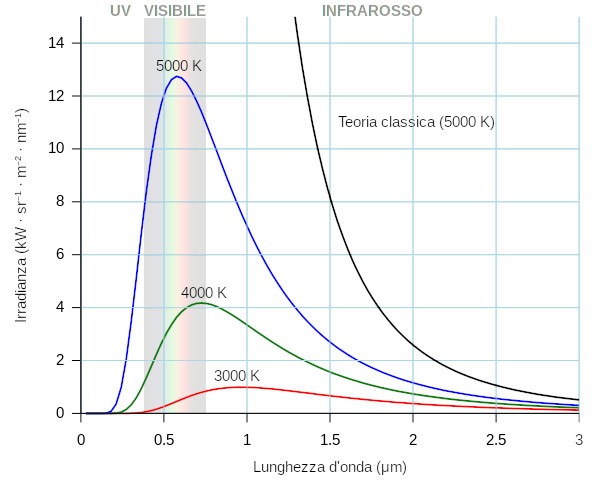
\includegraphics[width=.7\columnwidth]{parts/corponero.jpg}
% \caption{Dati sperimentali per la quantità di energia emessa nelle diverse lunghezze d'onda. L'area sottesa dalla curva fornisce l'energia totale emessa.}
% \label{img:radianza}
% \end{figure}
%  
% %   \begin{figure}[htpb]\centering
% %     \begin{tikzpicture}[samples=100, scale=1.2]
% %     \begin{axis}[
% %         xmin=0,
% %         xmax=30,
% %         xlabel={{\footnotesize $\lambda \, [nm]$}},
% %         ymin=0,
% %         ymax=pi,
% %         ylabel={{\footnotesize $\rho (\lambda; T) \, [\sfrac{W}{m^2}]$}},
% %         xtick=\empty,
% %         ytick=\empty,
% %         no markers,
% %         grid=both,domain=0.1:40,
% %         style={}]
% %         \fill [black!10] (2,0.005) rectangle (6,pi-0.005);
% %         \addplot[fill=colorSitoScuro,fill opacity=.25,thick,colorSitoScuro] {(x^3)/((pi^2)*(exp(2000*x/(3000))-1))};
% %         \addlegendentryexpanded{{\footnotesize $T = 3000 \, K$}}
% %         \addplot[fill=colorSito,fill opacity=.25,thick,colorSito] {(x^3)/((pi^2)*(exp(2000*x/(4000))-1))};
% %         \addlegendentryexpanded{{\footnotesize $T = 4000 \, K$}}
% %         \addplot[fill=colorSitoChiaro,fill opacity=.25,thick,colorSitoChiaro] {(x^3)/((pi^2)*(exp(2000*x/(5000))-1))};
% %         \addlegendentryexpanded{{\footnotesize $T = 5000 \, K$}}
% %         \addplot[thick,colorSitoChiaro!60,dashed,domain=9.5:40] {(12/((x-5.6))- .3)};
% %         \addlegendentryexpanded{{\footnotesize previsione classica}}
% %         \draw[black!30] (2,0.005)--(2,pi-0.005);
% %         \draw[black!30] (6,0.005)--(6,pi-0.005);
% %         \node[below] at (4,pi) {{\scriptsize visibile}};
% %         \node[below] at (1,pi) {{\scriptsize UV}};
% %         \node[below] at (7,pi) {{\scriptsize IR}};
% %     \end{axis}
% %     \end{tikzpicture}
% %   \caption{Dati sperimentali per la quantità di energia emessa nelle diverse lunghezze d'onda. L'area sottesa dalla curva fornisce l'energia totale emessa.}
% %   \label{img:radianza}
% %   \end{figure}
%   
%   \item[Legge di Wien] 
%   Fornisce la lunghezza d'onda per cui sia ha il picco di intensità di radiazione in funzione della temperatura.
%   \[ \lambda_{max} = \frac{0,2898}{T} \, cm \]
%   
%   \item[Legge di Stefan-Boltzmann] 
%   La radianza spettrale è la quantità di energia emessa dall'unità di superficie nell'unità di tempo.
%   \[ R_{sp} = \sigma T^4 \]
%   $ \sigma $ = costante di Stefan-Boltzmann = $ 5,6693 \times 10^{-8} \, \sfrac{W}{m^2 \cdot K^4} $
%   
%   \item[Costante di Planck]
%   \[ h = 6,62607 \times 10^{-34} \, J\cdot s \]
%   
%   \item[Energia trasportata dal campo elettromagnetico]
%   \[ E=nhf \]
%   $ n $ = numero intero positivo
%   
%   \item[Fotoni] 
%   Sono i \emph{quanti del campo elettromagnetico} e hanno massa nulla ed energia quantizzata pari a:
%   \[ E=hf \]
%   Anche la quantità di moto dei fotoni è quantizzata:
%   \[ p = \frac{E}{c} = \frac{hf}{c} \]
%   
%   \item[Effetto Compton] 
%   Inviando raggi X su un bersaglio di grafite la radiazione diffusa mostra, oltre ai raggi X con la stessa lunghezza d'onda, anche raggi con lunghezza d'onda maggiore.
%   \[ \Delta \lambda = \lambda' - \lambda = \frac{h}{m_e c} (1 - \cos \varphi) \]
%   \begin{multicols}{2}
%   $ m_e $ = massa dell'elettrone = $ 9,11 \times 10^{-31} \, kg $\\
%   $ \varphi  $ = angolo di diffusione del fotone
%   \end{multicols}
%   
%   \item[Serie di Balmer] 
%   Permette di calcolare le frequenze delle diverse onde elettromagnetiche emesse dall'atomo di idrogeno.
%   \[ f = c R_H \left( \frac{1}{m^2} - \frac{1}{n^2} \right) \]
%   $ R_H $ = costante di Rydberg dell'idrogeno = $ 1,097 \times 10^7 \, m^{-1}$\\
%   $ m $, $ n $ = numeri naturali, con $ n>m $
%   
%   \item[Esperimento di Millikan] 
%   Ha permesso di misurare la carica dell'elettrone, $ -e $:
%   \[ e = 1,602 \times 10^{-19} \, C \]
%   
%   \item[Principio di esclusione di Pauli] 
%   Su una stessa orbita non possono muoversi più di due elettroni.
%   
%   \item[Raggi delle orbite di Bohr]
%   \[ r_n = n^2 \cdot \frac{\varepsilon_0 h^2}{\pi m_e e^2} = (5,29 \times 10^{-11} \, m)\cdot n^2 \]
%   $ n $ = numero quantico principale
%   
%   \item[Relazione di De Broglie] 
%   Ad una particella con quantità di moto $ p $ è associata una lunghezza d'onda:
%   \[ \lambda = \frac{h}{p} \] Tale lunghezza d'onda è detta \emph{lunghezza d'onda di De Broglie} della particella.
%   
%   \item[Dualismo onda-particella] 
%   Sia la radiazione elettromagnetica sia le particelle subatomiche mostrano in alcuni fenomeni natura ondulatoria, in altri natura corpuscolare.
%   
%   \item[Costante di Planck ridotta] 
%   \[ \hbar = \frac{h}{2 \pi} \simeq 10^{-34} \, J\cdot s \]
%   
%   \item[Principio di indeterminazione di Heisenberg] 
%   Può essere formulato in due modi equivalenti: 
%   \[ \Delta x \Delta p \simeq \hbar \]
%   \[ \Delta t \Delta E \simeq \hbar \]
%   Non è possibile conoscere con precisione dove l'elettrone si trova senza impartirgli una quantità di moto non determinabile. Inoltre, più breve è la misura dell'energia effettuata su un sistema, più impreciso è il valore dell'energia misurato.
%   
%   \item[Funzione d'onda $ \mathbf{\Psi} $]
%   È la soluzione dell'equazione di Schrödinger del sistema in esame. Esprime un'ampiezza di probabilità e dipende dalle tre componenti spaziali e da quella temporale.
%   
%   Permette di calcolare la probabilità che la particella alla quale è associata si trovi in un volume di spazio in un certo intervallo di tempo.
%   
%   La probabilità di osservare la particella è proporzionale al quadrato di $ \Psi $.
% \end{description}
%

% \newpage
% \section{Derivate e integrali notevoli}
%
% \begin{description}
%   \item[Variazioni istantanee e velocità]
%   La derivata della funzione $ f $ rispetto alla variabile $ x $ è definita come:
%   \[ f'(x) = \lim_{\Delta x \to 0} \frac{\Delta f}{\Delta x} = \frac{df}{dx} \]
%   Intuitivamente, la derivata di una funzione in un punto fornisce indicazioni sulla \emph{velocità di variazione} della funzione in quel punto.
%   
%   Tale informazione viene espressa graficamente dal coefficiente angolare della retta tangente al grafico della funzione in quel punto.
%   
%   \item[Notazioni per la derivata di una funzione]
%   Possiamo indicare la derivata (prima e seconda) della funzione $ f $ rispetto alla variabile $ x $ in diversi modi, in base alla comodità e al contesto, come indicato in \Cref{tab:scritturaderivate}.
%   
%   \begin{table}[htp]\centering
%   \begin{tabular}{ccc}\toprule
%     ~~~~\textbf{Lagrange}~~~~ & ~~~~\textbf{Leibniz}~~~~ & ~~~~\textbf{Eulero}~~~~ \\\midrule
%     $ f'(x),f''(x) $ & $ \dfrac{df}{dx},\dfrac{d^2 f}{dx^2} $ & $ D[f], D^2[f] $ \\\bottomrule
%   \end{tabular}
%   \caption{Tre modi diversi di esprimere la derivata prima e seconda di $ f(x) $.}
%   \label{tab:scritturaderivate}
%   \end{table}
%   
%   \item[Derivata temporale]
%   La derivata di una funzione avente come variabile il tempo è detta \emph{derivata temporale} di quella funzione.
%   
%   \item[Derivate e cinematica]
%   La funzione che esprime la posizione di un corpo nel \textsc{sdr} in funzione del tempo, la sua velocità istantanea e la sua accelerazione istantanea sono l'una la derivata (temporale) dell'altra.
%   
%   \[ s'(t) = \displaystyle \lim_{\Delta t \to 0} \frac{\Delta s}{\Delta t} = \frac{ds}{dt} = v(t) \]
%   
%   \[ s''(t) = v'(t) = \displaystyle \lim_{\Delta t \to 0} \frac{\Delta v}{\Delta t} = \frac{dv}{dt} = a(t) \]
%   
%   Possiamo verificare facilmente quanto detto per tutte le leggi orarie fornite alla \Cref{sec:cinematica}.
%   
%   \item[Derivate notevoli]
%   In \Cref{tab:derivatenotevoli} sono mostrate le quantità (istantanee) che possono essere ottenute derivando.
%   
%   \begin{table}[hbtp]\centering
%   \begin{tabular}{llll}\toprule
%     \textbf{Funzione} & \textbf{Derivata di} & \textbf{Rispetto a} & \textbf{Formula} \\\midrule
%     velocità          & posizione            & tempo               & $ v(t) = \dfrac{ds}{dt} $ \\\addlinespace[.8em]
%     accelerazione     & velocità             & tempo               & $ a(t) = \dfrac{dv}{dt} $ \\\addlinespace[.8em]
%     forza             & quantità di moto     & tempo               & $ F(t) = \dfrac{dp}{dt} $ \\\addlinespace[.8em]
%     forza             & energia              & posizione           & $ F(s) = \dfrac{dU}{ds} $ \\\addlinespace[.8em]
%     intensità di corrente & carica           & tempo               & $ i(t) = \dfrac{dq}{dt} $ \\\addlinespace[.8em]
%     potenza           & energia              & tempo               & $ P(t) = \dfrac{dU}{dt} $ \\\addlinespace[.8em]
%     $ \textrm{f}_{\textrm{em}} $ & flusso di $ B $ & tempo         & $ f_{em}(t) = -\dfrac{d\Phi(B)}{dt} $ \\\bottomrule
%   \end{tabular}
%   \caption{Alcune derivate notevoli.}
%   \label{tab:derivatenotevoli}
%   \end{table}
%   
%   \item[Spazio percorso]
%   Conoscendo la funzione $ v(t) $ che esprime la velocità di un corpo in funzione del tempo, 
%   possiamo calcolare lo spazio percorso tra un tempo $ t_0 $ e un tempo $ t_1 $ con:
%   \[ \Delta s = \int_{t_0}^{t_1} v dt \]
%   Questo integrale definito fornisce l'area sottesa dal grafico di $ v(t) $ tra il tempo $ t_0 $ e il tempo $ t_1 $.
%   
%   \item[Lavoro di una forza]
%   Conoscendo la funzione $ F(s) $ che esprime la forza agente su un corpo in funzione della sua posizione, 
%   possiamo calcolare il lavoro di tale forza (e quindi la variazione di energia potenziale del corpo) tra la posizione $ s_0 $ e la posizione $ s_1 $ con:
%   \[ L = \Delta U = \int_{s_0}^{s_1} F(s) ds \]
%   
%   \item[Circuitazione] Alle \cpageref{conc:circuitazioneE,conc:circuitazioneB} abbiamo definito la circuitazione lungo la linea chiusa $ \mathscr{L} $ 
%   come una sommatoria di prodotti scalari tra un vettore campo e un vettore spostamento (cioè tutti gli spostamenti necessari per percorrere $ \mathscr{L} $). 
%   
%   Possiamo pertanto esprimere la circuitazione (del campo elettrico o magnetico) con:
%   \begin{multicols}{2}
%   \begin{center}
%   $ \displaystyle \Gamma_\mathscr{L}(E) = \oint_\mathscr{L} \vec{E} \cdot d\vec{\ell} $
%   
%   $ \displaystyle \Gamma_\mathscr{L}(B) = \oint_\mathscr{L} \vec{B} \cdot d\vec{\ell} $
%   \end{center}
%   \end{multicols}
%   Il simbolo $ \oint_\mathscr{L} $ indica l'integrale chiuso sulla linea $ \mathscr{L} $.
% \end{description}
%
%

\newpage
\section{Timeline}
\begin{turn}{90}
\begin{minipage}{\linewidth}
\scalebox{.66}{\hspace*{-12cm}\begin{timeline}[min=1550,max=2000,step=25]
\tlbar{1548}{1620}{Stevino}
\tlbar{1564}{1642}{Galileo}
\tlbar{1571}{1630}{Keplero}
\tlbar{1596}{1650}{Cartesio}
\tlbar{1608}{1647}{Torricelli}
\tlbar{1623}{1662}{Pascal}
\tlbar{1627}{1691}{Boyle}
\tlbar{1629}{1695}{Huygens}
\tlbar{1635}{1703}{Hooke}
\tlbar{1643}{1727}{Newton}
\tlbar{1736}{1806}{Coulomb}
\tlbar{1736}{1819}{Watt}
\tlbar{1743}{1794}{Lavoisier}
\tlbar{1745}{1827}{Volta}
\tlbar{1766}{1844}{Dalton}
\tlbar{1775}{1836}{Ampère}
\tlbar{1777}{1851}{Oersted}
\tlbar{1777}{1855}{Gauss}
\tlbar{1778}{1850}{Gay-Lussac}
\tlbar{1789}{1854}{Ohm}
\tlbar{1791}{1867}{Faraday}
\tlbar{1796}{1832}{Carnot}
\tlbar{1818}{1889}{Joule}
\tlbar{1824}{1907}{Kelvin}
\tlbar{1831}{1879}{Maxwell}
\tlbar{1834}{1907}{Mendeleev}
\tlbar{1844}{1906}{Boltzmann}
\tlbar{1856}{1940}{Thomson}
\tlbar{1856}{1943}{Tesla}
\tlbar{1857}{1894}{Hertz}
\tlbar{1858}{1947}{Planck}
\tlbar{1871}{1937}{Rutherford}
\tlbar{1879}{1955}{Einstein}
\tlbar{1885}{1962}{Bohr}
\tlbar{1887}{1961}{Schrödinger}
\tlbar{1891}{1987}{De Broglie}
\tlbar{1901}{1954}{Fermi}
\tlbar{1901}{1976}{Heisenberg}
\end{timeline}
}
\end{minipage}
\end{turn}

\newpage
\section{Tavola periodica degli elementi}
	~
	
	~
	
	\newcommand{\NaturalElementTextFormat}[7]
	{
		\begin{minipage}{2.21cm}
			\centering
			{\textbf{#1}\hspace{1em} \underline{{#7}} \hfill {#2}\textit{{#3}}}%
			\\[0.1cm]
			{\Huge \textbf{{#5}}}
			\linebreak
			{\fontsize{9.5}{10.0}\selectfont {#6} }
			\linebreak
			{\small {#4}} 
		\end{minipage}
	}
	
	\newcommand{\KeyTextFormat}[7]
	{
		\begin{minipage}{2.21m}
			\centering
			{\textbf{#1}\hspace{1em} \underline{{#7}} \hfill {#2}\textit{{#3}}}%
			\\[0.1cm]
			{\Huge \textbf{{#5}}}
			\linebreak
			{\fontsize{9.5}{10}\selectfont {#6} }
			\linebreak
			{\small {#4}} 
		\end{minipage}
	}
	\tikzstyle{SBlock} = [fill=colorSitoChiaro!15] %primo+elio
	\tikzstyle{PBlock} = [fill=colorSitoScuro!5] %terzo
	\tikzstyle{DBlock} = [fill=colorSito!30] %secondo
	\tikzstyle{FBlock} = [fill=colorSitoScuro!35] %altri
	
	\begin{tikzpicture}[scale=0.4633, transform shape, rotate=90]
	
	\tikzstyle{KeyBox} =  [draw=black, minimum width=2.4cm, minimum height=2.4cm, node distance=2.4cm, inner sep=0pt]
	\tikzstyle{Element} = [draw=black, minimum width=2.4cm, minimum height=2.4cm, node distance=2.4cm, inner sep=0pt]
	\tikzstyle{Offsetter} = [draw=white, minimum width=2.4cm, minimum height=2.4cm, node distance=2.4cm, inner sep=0pt]
	\tikzstyle{TitleLabel} = [font={\Huge\bfseries}]
	\tikzstyle{KeysLabel} = [minimum height = 2.5cm, inner sep=0pt, text width = 10cm]
	\tikzstyle{DetailsLabel} = [minimum height = 2.5cm, node distance = 2.5cm, inner sep=0pt]
	
	%% Group 1 - IA
	\node[name=Blank1, Offsetter] {}; % this is just an invisible box that shoves the entire table downward to make it more centered
	\node[name=Blank2, below of=Blank1, Offsetter] {}; % see comment on invisible box above.
	\node[name=H,	below of=Blank2, SBlock, Element] {\NaturalElementTextFormat{1}{}{}{1.00784}{H}{Idrogeno}{}};
	\node[name=Li, 	below of=H, 	SBlock, Element] {\NaturalElementTextFormat{3}{}{}{6.938}{Li}{Litio}{}};
	\node[name=Na, 	below of=Li,	SBlock, Element] {\NaturalElementTextFormat{11}{}{}{22.98976928}{Na}{Sodio}{}};
	\node[name=K, 	below of=Na,	SBlock, Element] {\NaturalElementTextFormat{19}{}{}{39.0983}{K}{Potassio}{}};
	\node[name=Rb, 	below of=K, 	SBlock, Element] {\NaturalElementTextFormat{37}{}{}{85.4678}{Rb}{Rubidio}{}};
	\node[name=Cs, 	below of=Rb,	SBlock, Element] {\NaturalElementTextFormat{55}{}{}{132.90545196}{Cs}{Cesio}{}};
	\node[name=Fr, 	below of=Cs,	SBlock, Element] {\NaturalElementTextFormat{87}{}{}{(223)}{Fr}{Francio}{}};
	
	%% Group 2 - IIA
	\node[name=Be, right of=Li, SBlock, Element] {\NaturalElementTextFormat{4}{}{}{9.0121831}{Be}{Berillio}{}};
	\node[name=Mg, below of=Be, SBlock, Element] {\NaturalElementTextFormat{12}{}{}{24.304}{Mg}{Magnesio}{}};
	\node[name=Ca, below of=Mg, SBlock, Element] {\NaturalElementTextFormat{20}{}{}{40.078}{Ca}{Calcio}{}};
	\node[name=Sr, below of=Ca, SBlock, Element] {\NaturalElementTextFormat{38}{}{}{87.62}{Sr}{Stronzio}{}};
	\node[name=Ba, below of=Sr, SBlock, Element] {\NaturalElementTextFormat{56}{}{}{137.327}{Ba}{Bario}{}};
	\node[name=Ra, below of=Ba, SBlock, Element] {\NaturalElementTextFormat{88}{}{}{(226)}{Ra}{Radio}{}};
	
	%% Group 3 - IIIB
	\node[name=Sc, 	right of=Ca, 	DBlock,  Element] {\NaturalElementTextFormat{21}{}{}{44.955908}{Sc}{Sandio}{}};
	\node[name=Y, 	below of=Sc, 	DBlock, Element] {\NaturalElementTextFormat{39}{}{}{88.90584}{Y}{Ittirio}{}};
	\node[name=LaLu, 	below of=Y, 	Element] {\NaturalElementTextFormat{57-71}{}{}{}{*}{Lantanidi}{}};
	\node[name=AcLr, 	below of=LaLu, 	Element] {\NaturalElementTextFormat{89-103}{}{}{}{**}{Attinidi}{}};
	
	%% Group 4 - IVB
	\node[name=Ti, right of=Sc, DBlock, Element] {\NaturalElementTextFormat{22}{}{}{47.867}{Ti}{Titanio}{}};
	\node[name=Zr, below of=Ti,DBlock,  Element] {\NaturalElementTextFormat{40}{}{}{91.224}{Zr}{Zirconio}{}};
	\node[name=Hf, below of=Zr,DBlock,  Element] {\NaturalElementTextFormat{72}{}{}{178.49}{Hf}{Afnio}{}};
	\node[name=Rf, below of=Hf, DBlock, Element] {\NaturalElementTextFormat{104}{}{}{(261)}{Rf}{Rutherfordio}{}};
	
	%% Group 5 - VB
	\node[name=V, right of=Ti, DBlock, Element] {\NaturalElementTextFormat{23}{}{}{50.9415}{V}{Vanadio}{}};
	\node[name=Nb, below of=V, DBlock, Element] {\NaturalElementTextFormat{41}{}{}{92.90637}{Nb}{Niobio}{}};
	\node[name=Ta, below of=Nb, DBlock, Element] {\NaturalElementTextFormat{73}{}{}{180.94788}{Ta}{Tantalio}{}};
	\node[name=Db, below of=Ta, DBlock, Element] {\NaturalElementTextFormat{105}{}{}{(268)}{Db}{Dubnio}{}};
	
	%% Group 6 - VIB
	\node[name=Cr, right of=V, DBlock, Element] {\NaturalElementTextFormat{24}{}{}{51.9961}{Cr}{Cromo}{}};
	\node[name=Mo, below of=Cr,DBlock,  Element] {\NaturalElementTextFormat{42}{}{}{95.95}{Mo}{Molibdeno}{}};
	\node[name=W, below of=Mo,DBlock,  Element] {\NaturalElementTextFormat{74}{}{}{183.84}{W}{Tungsteno}{}};
	\node[name=Sg, below of=W, DBlock, Element] {\NaturalElementTextFormat{106}{}{}{(269)}{Sg}{Seaborgio}{}};
	
	%% Group 7 - VIIB
	\node[name=Mn, right of=Cr, DBlock, Element] {\NaturalElementTextFormat{25}{}{}{54.938044}{Mn}{Manganese}{}};
	\node[name=Tc, below of=Mn, DBlock, Element] {\NaturalElementTextFormat{43}{}{}{(98)}{Tc}{Tecnezio}{}};
	\node[name=Re, below of=Tc, DBlock, Element] {\NaturalElementTextFormat{75}{}{}{186.207}{Re}{Renio}{}};
	\node[name=Bh, below of=Re, DBlock, Element] {\NaturalElementTextFormat{107}{}{}{(270)}{Bh}{Bohrio}{}};
	
	%% Group 8 - VIIIB
	\node[name=Fe, right of=Mn, DBlock, Element] {\NaturalElementTextFormat{26}{}{}{55.845}{Fe}{Ferro}{}};
	\node[name=Ru, below of=Fe, DBlock, Element] {\NaturalElementTextFormat{44}{}{}{101.07}{Ru}{Rutenio}{}};
	\node[name=Os, below of=Ru, DBlock, Element] {\NaturalElementTextFormat{76}{}{}{190.23}{Os}{Osmio}{}};
	\node[name=Hs, below of=Os, DBlock, Element] {\NaturalElementTextFormat{108}{}{}{(269)}{Hs}{Hassio}{}};
	
	%% Group 9 - VIIIB
	\node[name=Co, right of=Fe,DBlock,  Element] {\NaturalElementTextFormat{27}{}{}{58.933194}{Co}{Cobalto}{}};
	\node[name=Rh, below of=Co, DBlock, Element] {\NaturalElementTextFormat{45}{}{}{102.90550}{Rh}{Rodio}{}};
	\node[name=Ir, below of=Rh, DBlock, Element] {\NaturalElementTextFormat{77}{}{}{192.217}{Ir}{Iridio}{}};
	\node[name=Mt, below of=Ir, DBlock, Element] {\NaturalElementTextFormat{109}{}{}{(278)}{Mt}{Meitnerio}{}};
	
	%% Group 10 - VIIIB
	\node[name=Ni, right of=Co, DBlock, Element] {\NaturalElementTextFormat{28}{}{}{58.6934}{Ni}{Nichel}{}};
	\node[name=Pd, below of=Ni, DBlock, Element] {\NaturalElementTextFormat{46}{}{}{106.42}{Pd}{Palladio}{}};
	\node[name=Pt, below of=Pd, DBlock, Element] {\NaturalElementTextFormat{78}{}{}{195.084}{Pt}{Platino}{}};
	\node[name=Ds, below of=Pt, DBlock, Element] {\NaturalElementTextFormat{110}{}{}{(281)}{Ds}{Darmstadio}{}};
	
	%% Group 11 - IB
	\node[name=Cu, right of=Ni, DBlock, Element] {\NaturalElementTextFormat{29}{}{}{63.546(3)}{Cu}{Rame}{}};
	\node[name=Ag, below of=Cu, DBlock, Element] {\NaturalElementTextFormat{47}{}{}{107.8682(2)}{Ag}{Argento}{}};
	\node[name=Au, below of=Ag, DBlock, Element] {\NaturalElementTextFormat{79}{}{}{196.966569(5)}{Au}{Oro}{}};
	\node[name=Rg, below of=Au,DBlock,  Element] {\NaturalElementTextFormat{111}{}{}{(282)}{Rg}{Roentgenio}{}};
	
	%% Group 12 - IIB
	\node[name=Zn, right of=Cu, DBlock, Element] {\NaturalElementTextFormat{30}{}{}{65.38}{Zn}{Zinco}{}};
	\node[name=Cd, below of=Zn, DBlock, Element] {\NaturalElementTextFormat{48}{}{}{112.414}{Cd}{Cadmio}{}};
	\node[name=Hg, below of=Cd, DBlock, Element] {\NaturalElementTextFormat{80}{}{}{200.592}{Hg}{Mercurio}{}};
	\node[name=Uub, below of=Hg, DBlock, Element] {\NaturalElementTextFormat{112}{}{}{(285)}{Cn}{Copernicio}{}};
	
	%% Group 13 - IIIA
	\node[name=Ga, right of=Zn, PBlock,  Element] {\NaturalElementTextFormat{31}{}{}{69.723}{Ga}{Gallio}{}};
	\node[name=Al, above of=Ga, PBlock,  Element] {\NaturalElementTextFormat{13}{}{}{26.9815385}{Al}{Alluminio}{}};
	\node[name=B, above of=Al, PBlock, Element] {\NaturalElementTextFormat{5}{}{}{10.806}{B}{Boro}{}};
	\node[name=In, below of=Ga, PBlock,  Element] {\NaturalElementTextFormat{49}{}{}{114.818}{In}{Indio}{}};
	\node[name=Tl, below of=In, PBlock,  Element] {\NaturalElementTextFormat{81}{}{}{204.382}{Tl}{Tallio}{}};
	\node[name=Uut, below of=Tl, PBlock,  Element] {\NaturalElementTextFormat{113}{}{}{(286)}{Uut}{Ununtrio}{}};
	
	%% Group 14 - IVA
	\node[name=C, right of=B, PBlock, Element] {\NaturalElementTextFormat{6}{}{}{12.0096}{C}{Carbonio}{}};
	\node[name=Si, below of=C,PBlock,  Element] {\NaturalElementTextFormat{14}{}{}{28.084}{Si}{Silicio}{}};
	\node[name=Ge, below of=Si, PBlock, Element] {\NaturalElementTextFormat{32}{}{}{72.630}{Ge}{Germanio}{}};
	\node[name=Sn, below of=Ge,PBlock,  Element] {\NaturalElementTextFormat{50}{}{}{118.710}{Sn}{Stagno}{}};
	\node[name=Pb, below of=Sn, PBlock, Element] {\NaturalElementTextFormat{82}{}{}{207.2}{Pb}{Piombo}{}};
	\node[name=Uuq, below of=Pb,PBlock,  Element] {\NaturalElementTextFormat{114}{}{}{(289)}{Fl}{Flerovio}{}};
	
	%% Group 15 - VA
	\node[name=N, right of=C, PBlock,  Element] {\NaturalElementTextFormat{7}{}{}{14.00643}{N}{Azoto}{}};
	\node[name=P, below of=N, PBlock,  Element] {\NaturalElementTextFormat{15}{}{}{30.973761998}{P}{Fosforo}{}};
	\node[name=As, below of=P,PBlock,   Element] {\NaturalElementTextFormat{33}{}{}{74.921595}{As}{Arsenico}{}};
	\node[name=Sb, below of=As, PBlock,  Element] {\NaturalElementTextFormat{51}{}{}{121.760}{Sb}{Antimonio}{}};
	\node[name=Bi, below of=Sb, PBlock,  Element] {\NaturalElementTextFormat{83}{}{}{208.98040}{Bi}{Bismuto}{}};
	\node[name=Uup, below of=Bi,PBlock,   Element] {\NaturalElementTextFormat{115}{}{}{(289)}{Uup}{Ununpentio}{}};
	
	%% Group 16 - VIA
	\node[name=O, right of=N,PBlock,   Element] {\NaturalElementTextFormat{8}{}{}{15.99903}{O}{Ossigeno}{}};
	\node[name=S, below of=O, PBlock,  Element] {\NaturalElementTextFormat{16}{}{}{32.059}{S}{Zolfo}{}};
	\node[name=Se, below of=S, PBlock,  Element] {\NaturalElementTextFormat{34}{}{}{78.971}{Se}{Selenio}{}};
	\node[name=Te, below of=Se, PBlock,  Element] {\NaturalElementTextFormat{52}{}{}{127.60}{Te}{Tellurio}{}};
	\node[name=Po, below of=Te, PBlock,  Element] {\NaturalElementTextFormat{84}{}{}{(209)}{Po}{Polonio}{}};
	\node[name=Uuh, below of=Po, PBlock,  Element] {\NaturalElementTextFormat{116}{}{}{(293)}{Lv}{Livermorio}{}};
	
	%% Group 17 - VIIA
	\node[name=F, right of=O, PBlock,  Element] {\NaturalElementTextFormat{9}{}{}{18.998403163}{F}{Fluoro}{}};
	\node[name=Cl, below of=F, PBlock,  Element] {\NaturalElementTextFormat{17}{}{}{35.446}{Cl}{Cloro}{}};
	\node[name=Br, below of=Cl, PBlock,  Element] {\NaturalElementTextFormat{35}{}{}{79.901}{Br}{Bromo}{}};
	\node[name=I, below of=Br, PBlock,  Element] {\NaturalElementTextFormat{53}{}{}{126.90447}{I}{Iodio}{}};
	\node[name=At, below of=I,PBlock,   Element] {\NaturalElementTextFormat{85}{}{}{(210)}{At}{Astato}{}};
	\node[name=Uus, below of=At, PBlock,  Element] {\NaturalElementTextFormat{117}{}{}{(294)}{Uus}{Ununseptio}{}}; 
	
	%% Group 18 - VIIIA
	\node[name=Ne, right of=F, PBlock,  Element] {\NaturalElementTextFormat{10}{}{}{20.1797}{Ne}{Neon}{}};
	\node[name=He, above of=Ne,SBlock,  Element] {\NaturalElementTextFormat{2}{}{}{4.002602}{He}{Elio}{}};
	\node[name=Ar, below of=Ne, PBlock,  Element] {\NaturalElementTextFormat{18}{}{}{39.948}{Ar}{Argon}{}};
	\node[name=Kr, below of=Ar, PBlock,  Element] {\NaturalElementTextFormat{36}{}{}{83.798}{Kr}{Krypton}{}};
	\node[name=Xe, below of=Kr, PBlock,  Element] {\NaturalElementTextFormat{54}{}{}{131.293}{Xe}{Xenon}{}};
	\node[name=Rn, below of=Xe, PBlock,  Element] {\NaturalElementTextFormat{86}{}{}{(222)}{Rn}{Radon}{}};
	\node[name=Uuo, below of=Rn, PBlock,  Element] {\NaturalElementTextFormat{118}{}{}{(294)}{Uuo}{Ununoctio}{}}; 
	
	
	%% Lanthanide
	\node[name=La, below of=AcLr, DBlock, Element, yshift=-0.6cm] {\NaturalElementTextFormat{57}{}{}{138.90547(7)}{La}{Lantanio}{}};
	\node[name=Ce, right of=La, FBlock, Element] {\NaturalElementTextFormat{58}{}{}{140.116}{Ce}{Cerio}{}};
	\node[name=Pr, right of=Ce, FBlock, Element] {\NaturalElementTextFormat{59}{}{}{140.90766}{Pr}{{Praseodimio}}{}};
	\node[name=Nd, right of=Pr, FBlock, Element] {\NaturalElementTextFormat{60}{}{}{144.242}{Nd}{Neodimio}{}};
	\node[name=Pm, right of=Nd, FBlock, Element] {\NaturalElementTextFormat{61}{}{}{(145)}{Pm}{Promezio}{}};
	\node[name=Sm, right of=Pm, FBlock, Element] {\NaturalElementTextFormat{62}{}{}{150.36}{Sm}{Samario}{}};
	\node[name=Eu, right of=Sm, FBlock, Element] {\NaturalElementTextFormat{63}{}{}{151.964}{Eu}{Europio}{}};
	\node[name=Gd, right of=Eu, FBlock, Element] {\NaturalElementTextFormat{64}{}{}{157.25}{Gd}{Gadolinio}{}};
	\node[name=Tb, right of=Gd, FBlock, Element] {\NaturalElementTextFormat{65}{}{}{158.92535}{Tb}{Terbio}{}};
	\node[name=Dy, right of=Tb, FBlock, Element] {\NaturalElementTextFormat{66}{}{}{162.500}{Dy}{Disprosio}{}};
	\node[name=Ho, right of=Dy, FBlock, Element] {\NaturalElementTextFormat{67}{}{}{164.93033}{Ho}{Olmio}{}};
	\node[name=Er, right of=Ho, FBlock, Element] {\NaturalElementTextFormat{68}{}{}{167.259}{Er}{Erbio}{}};
	\node[name=Tm, right of=Er, FBlock, Element] {\NaturalElementTextFormat{69}{}{}{168.93422}{Tm}{Tulio}{}};
	\node[name=Yb, right of=Tm, FBlock, Element] {\NaturalElementTextFormat{70}{}{}{173.045}{Yb}{Itterbio}{}};
	\node[name=Lu, right of=Yb, FBlock, Element] {\NaturalElementTextFormat{71}{}{}{174.9668}{Lu}{Lutezio}{}};
	
	%% Actinide
	\node[name=Ac, below of=La, DBlock, Element] {\NaturalElementTextFormat{89}{}{}{(227)}{Ac}{Attinio}{}};
	\node[name=Th, right of=Ac, FBlock, Element] {\NaturalElementTextFormat{90}{}{}{232.0377}{Th}{Torio}{}};
	\node[name=Pa, right of=Th, FBlock, Element] {\NaturalElementTextFormat{91}{}{}{231.03588}{Pa}{Protoattinio}{}};
	\node[name=U, right of=Pa, FBlock, Element] {\NaturalElementTextFormat{92}{}{}{238.02891}{U}{Uranio}{}};
	\node[name=Np, right of=U, FBlock, Element] {\NaturalElementTextFormat{93}{}{}{(237)}{Np}{Nettunio}{}};
	\node[name=Pu, right of=Np, FBlock, Element] {\NaturalElementTextFormat{94}{}{}{(244)}{Pu}{Plutonio}{}};
	\node[name=Am, right of=Pu, FBlock, Element] {\NaturalElementTextFormat{95}{}{}{(243)}{Am}{Americio}{}};
	\node[name=Cm, right of=Am, FBlock, Element] {\NaturalElementTextFormat{96}{}{}{(247)}{Cm}{Curio}{}};
	\node[name=Bk, right of=Cm, FBlock, Element] {\NaturalElementTextFormat{97}{}{}{(247)}{Bk}{Berkelio}{}};
	\node[name=Cf, right of=Bk, FBlock,  Element] {\NaturalElementTextFormat{98}{}{}{(251)}{Cf}{Californio}{}};
	\node[name=Es, right of=Cf, FBlock, Element] {\NaturalElementTextFormat{99}{}{}{(252)}{Es}{Einsteinio}{}};
	\node[name=Fm, right of=Es, FBlock, Element] {\NaturalElementTextFormat{100}{}{}{(257)}{Fm}{Fermio}{}};
	\node[name=Md, right of=Fm, FBlock, Element] {\NaturalElementTextFormat{101}{}{}{(258)}{Md}{Mendelevio}{}};
	\node[name=No, right of=Md, FBlock, Element] {\NaturalElementTextFormat{102}{}{}{(259)}{No}{Nobelio}{}};
	\node[name=Lr, right of=No, FBlock, Element] {\NaturalElementTextFormat{103}{}{}{(266)}{Lr}{Laurenzio}{}};
	\node[name=Star, left of=La, Offsetter, xshift=-0.1cm] {{\textbf{\Huge *}}};
	\node[name=DoubleStar, below of=Star, Offsetter] {{\textbf{\Huge **}}};
	
	\node[name=Key, above of=Ti, Element, yshift=2.3cm] {\NaturalElementTextFormat{Z}{}{}{mass}{Sim}{Nome}{}};
	\node[above of=Mn, name=keyvalues, KeysLabel, yshift=3.8cm]{Z = numero atomico\\Sim = simbolo\\Nome = nome dell'elemento\\mass = massa atomica standard in \emph{unità di massa atomica}};
	\end{tikzpicture}



\end{document}
